\thispagestyle{toancuabinone}
\pagestyle{toancuabi}
\everymath{\color{toancuabi}}
%\blfootnote{$^1$\color{toancuabi}Đại học Thăng Long.}
\graphicspath{{../toancuabi/pic/}}
\begingroup
\AddToShipoutPicture*{\put(0,616){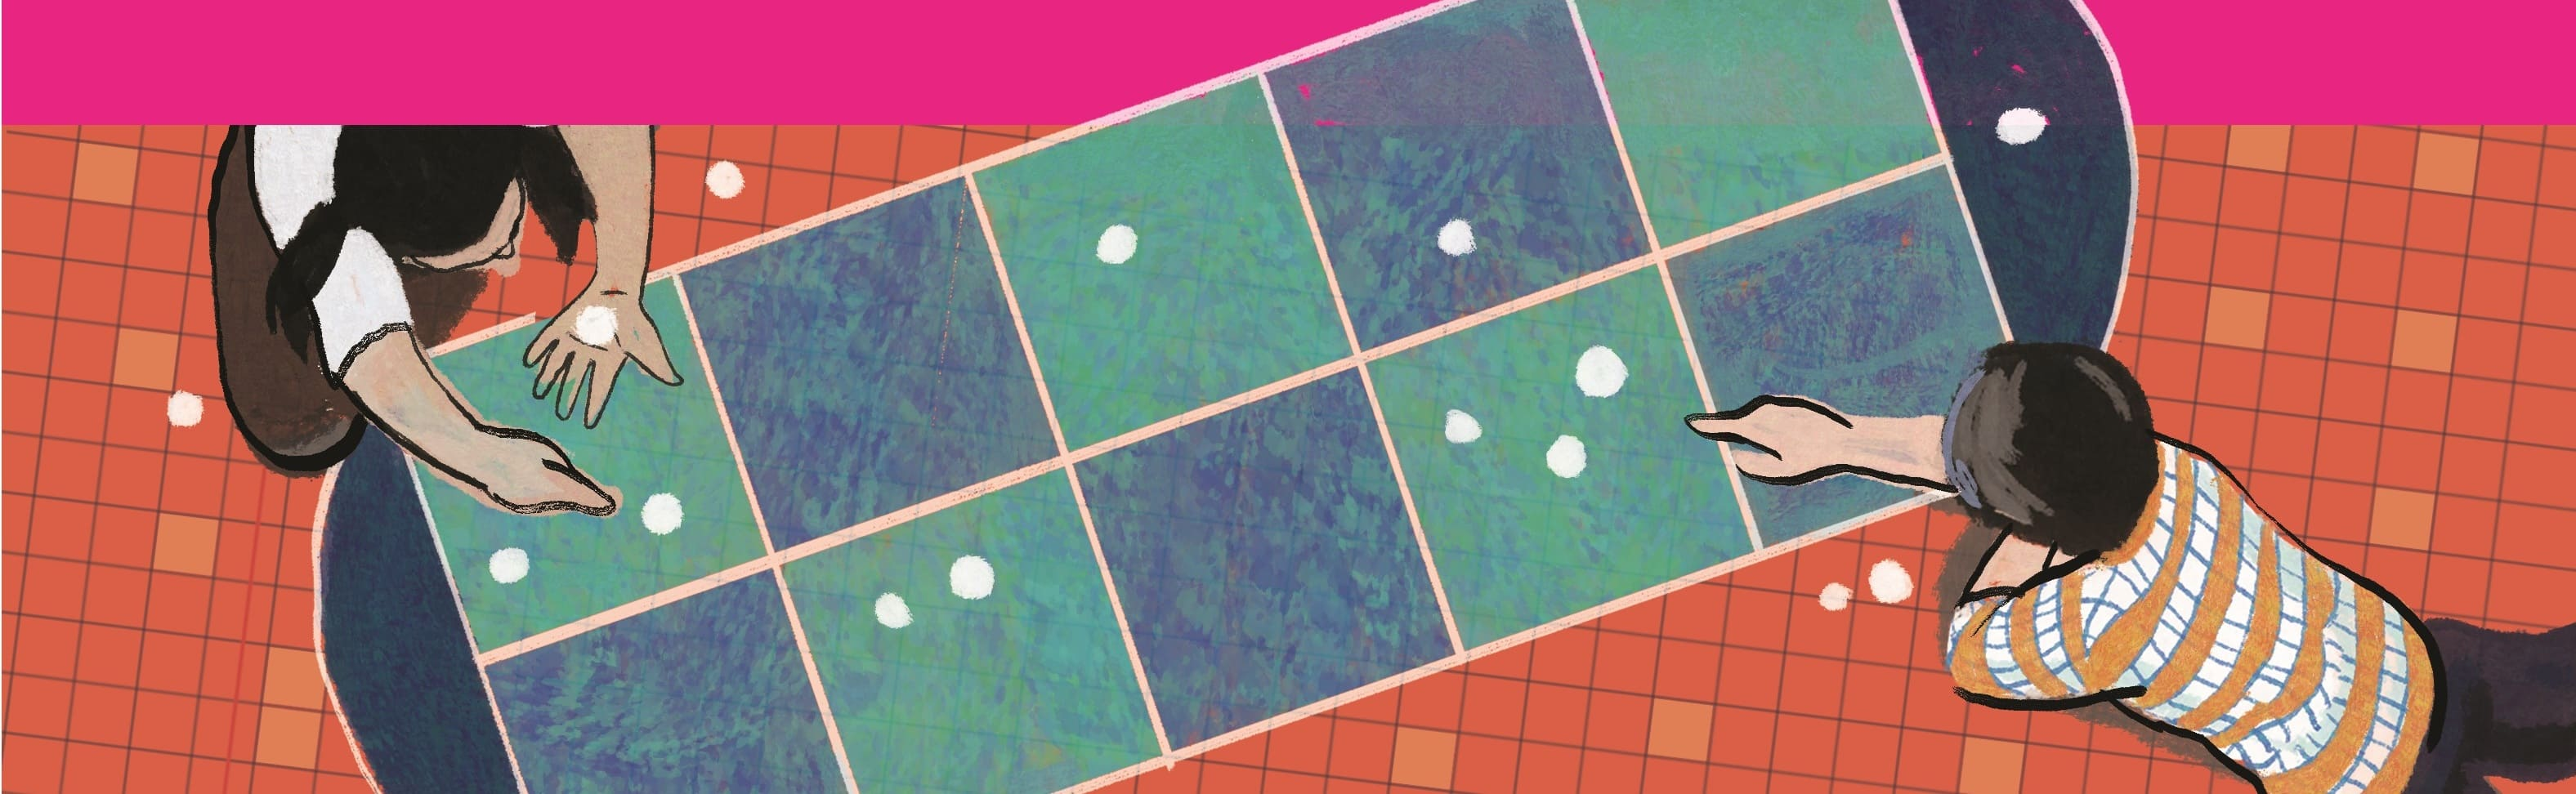
\includegraphics[width=19.3cm]{../bannertoancuabi}}}  
\AddToShipoutPicture*{\put(130,555){
\includegraphics[scale=1]{../tieude.pdf}}} 
\centering
\endgroup
\vspace*{150pt}

\begin{multicols}{2}
	Lần này thì Thám tử Xuân Phong phải vào tận hang ổ của một băng đảng để điều tra manh mối về một vụ án. Khác với những lần bị lạc lên đảo, ở đó có những thổ dân nói thật hoặc nói dối, trong ba người thuộc  băng đảng mà Xuân Phong tiếp cận, không có ai nói thật mà lại có tới ba kiểu người. Loại thứ nhất, tất nhiên rồi, đó là người Nói dối -- chuyên nói sai sự thật. Tiếp theo mới phức tạp cho Xuân Phong, lại có kẻ Ranh mãnh: hắn sẽ nói thật hoặc nói dối bất cứ khi nào hắn muốn. Thế chưa hết, loại cuối cùng mới rầy rà, đó là người Thay đổi, cứ nói thật và nói dối luân phiên nhau. Nhiệm vụ của Thám tử là xác định  từng người thuộc kiểu gì. Vừa được miêu tả về ba kiểu người như vậy, thanh tra Lê Kính đã ôm đầu kêu rên: ``Thôi, thà cho tôi lên hoang đảo với thổ dân nói Thật và nói Dối rõ ràng còn hơn. Ở đây phức tạp tờ mờ quá, không biết đường nào mà lần!"
	\vskip 0.1cm
	Xuân Phong đưa tay trấn an sự bực tức nóng nảy của thanh tra Lê Kính, thì thầm nói: ``Anh cứ yên tâm. Thế giới của băng đảng này phức tạp như vậy, nhưng tôi quả quyết chỉ sau không quá ba câu hỏi, ta sẽ biết ngay ai là thuộc loại người nào?"
	\vskip 0.1cm
	Làm thế nào mà Xuân Phong lại tự tin như thế nhỉ? Em có thể tìm thấy cách Thám tử đặt câu hỏi để xác định ai là ai, và giúp Lê Kính lấy lại bình tĩnh hay không?
\end{multicols}
\begin{figure}[H]
	\centering
	\vspace*{-5pt}
	\captionsetup{labelformat= empty, justification=centering}
	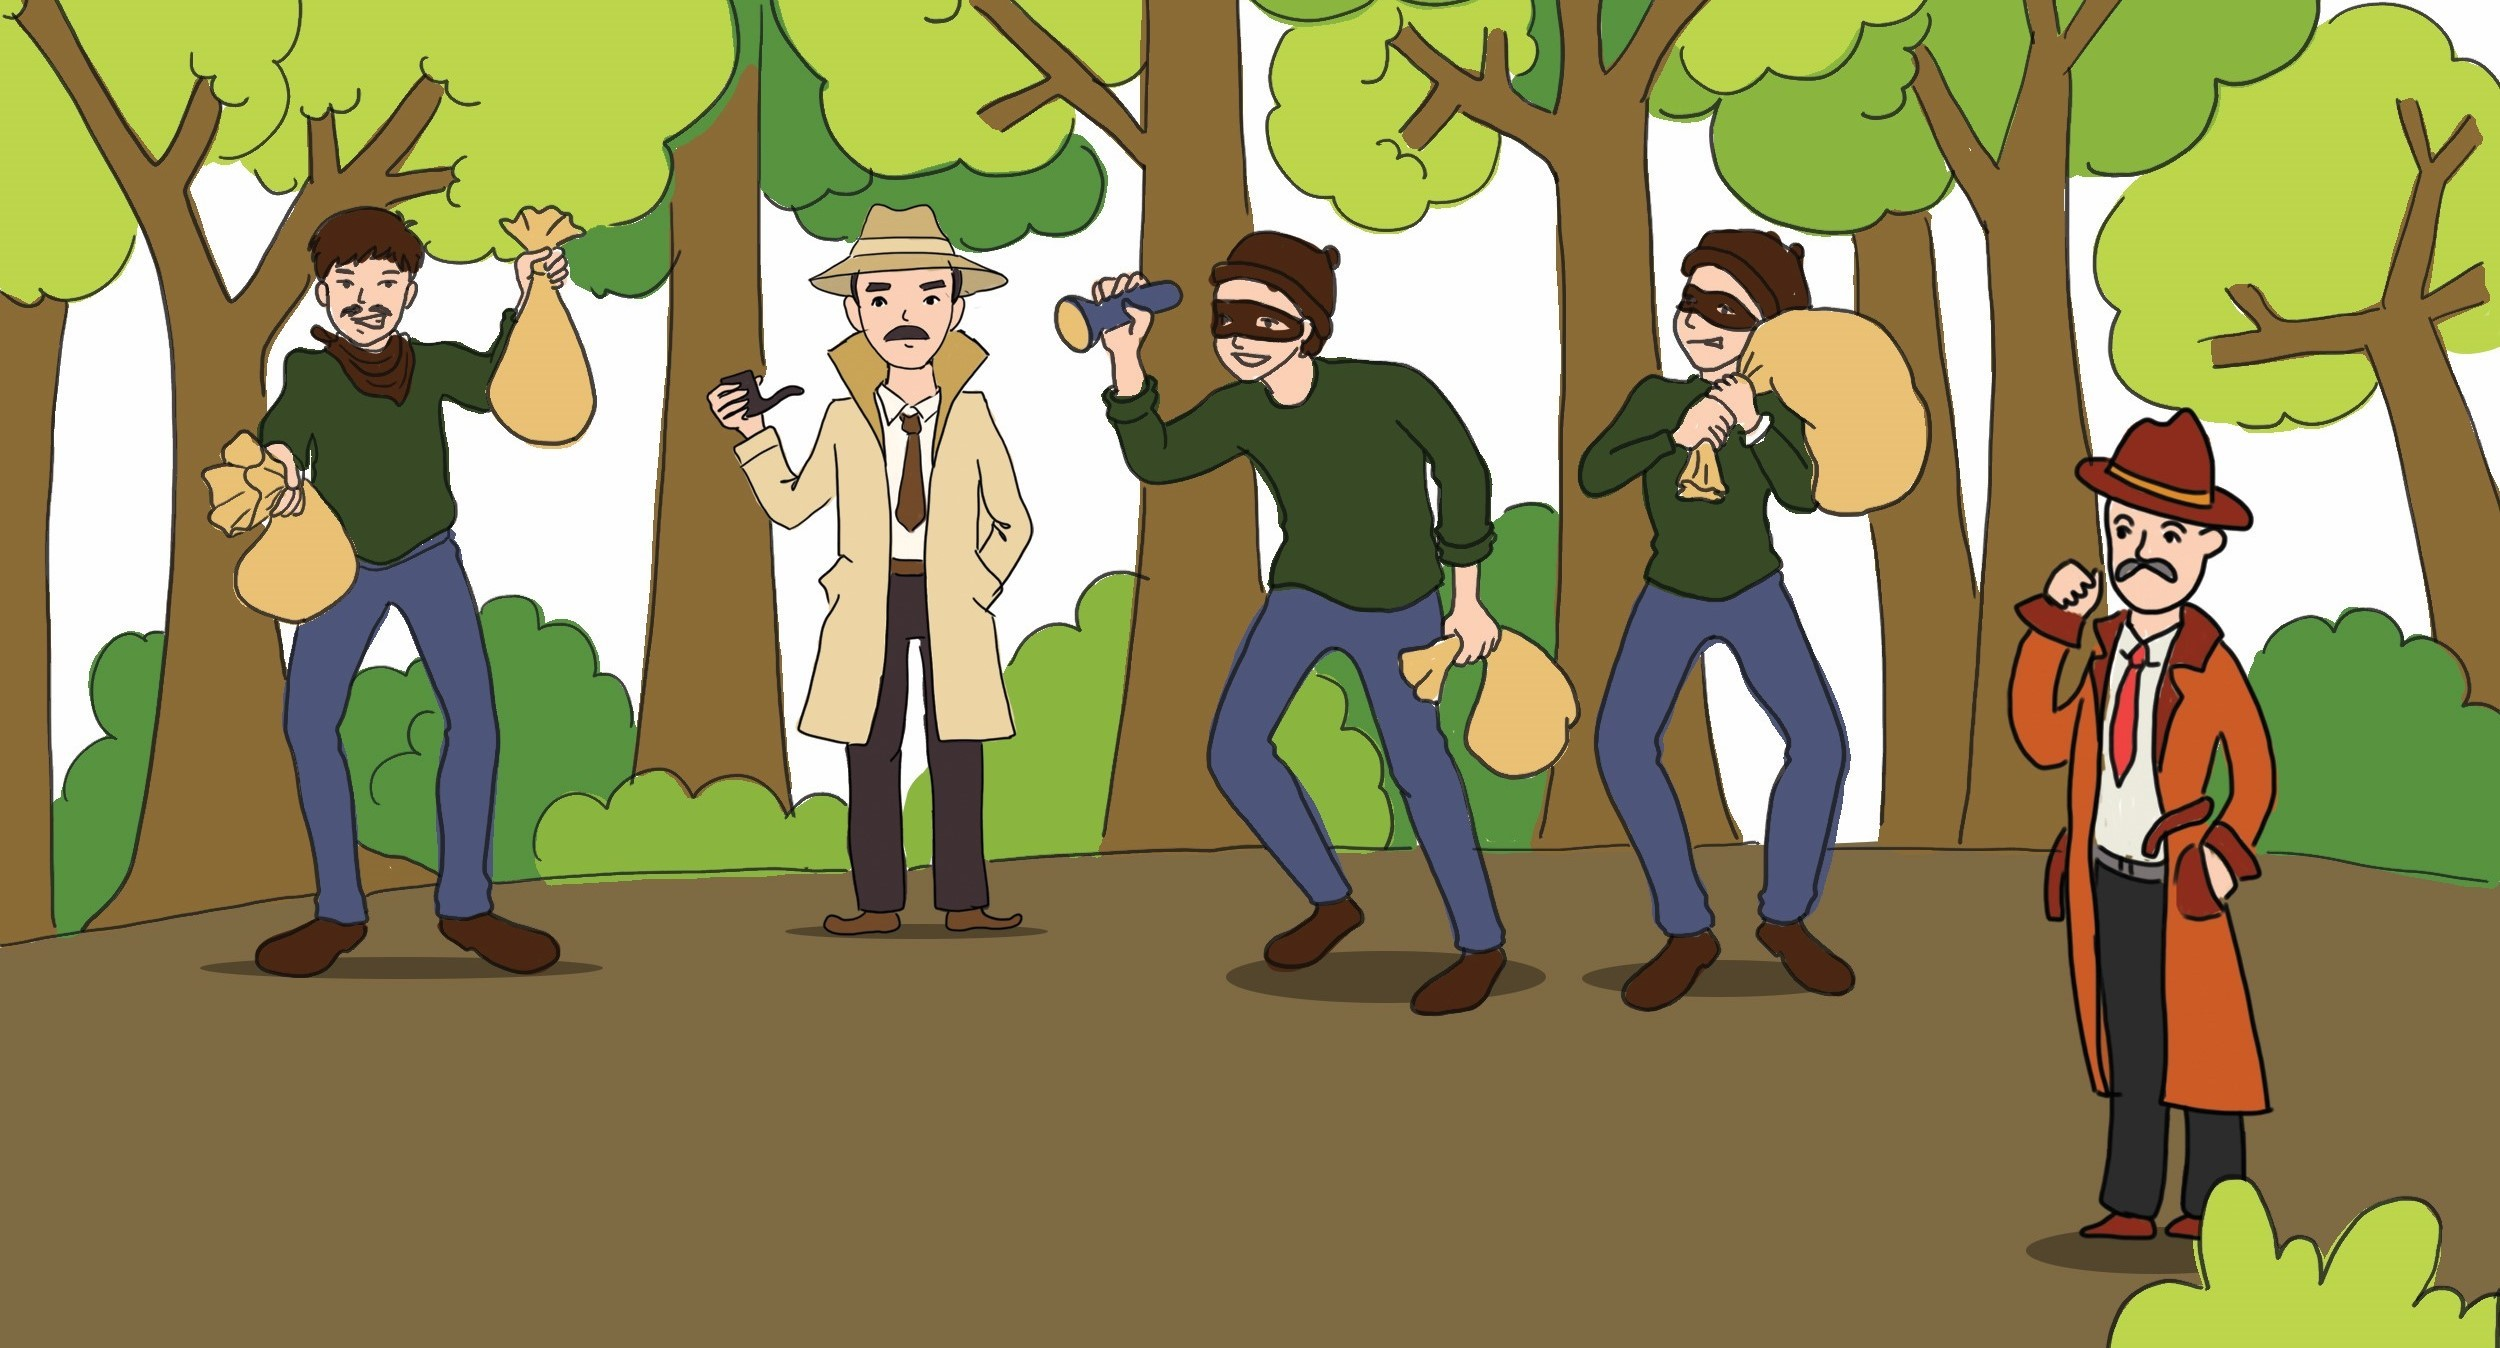
\includegraphics[width=1\linewidth]{xuanphong}
	\vspace*{-10pt}
\end{figure}
\newpage
\begingroup
\AddToShipoutPicture*{\put(115,670){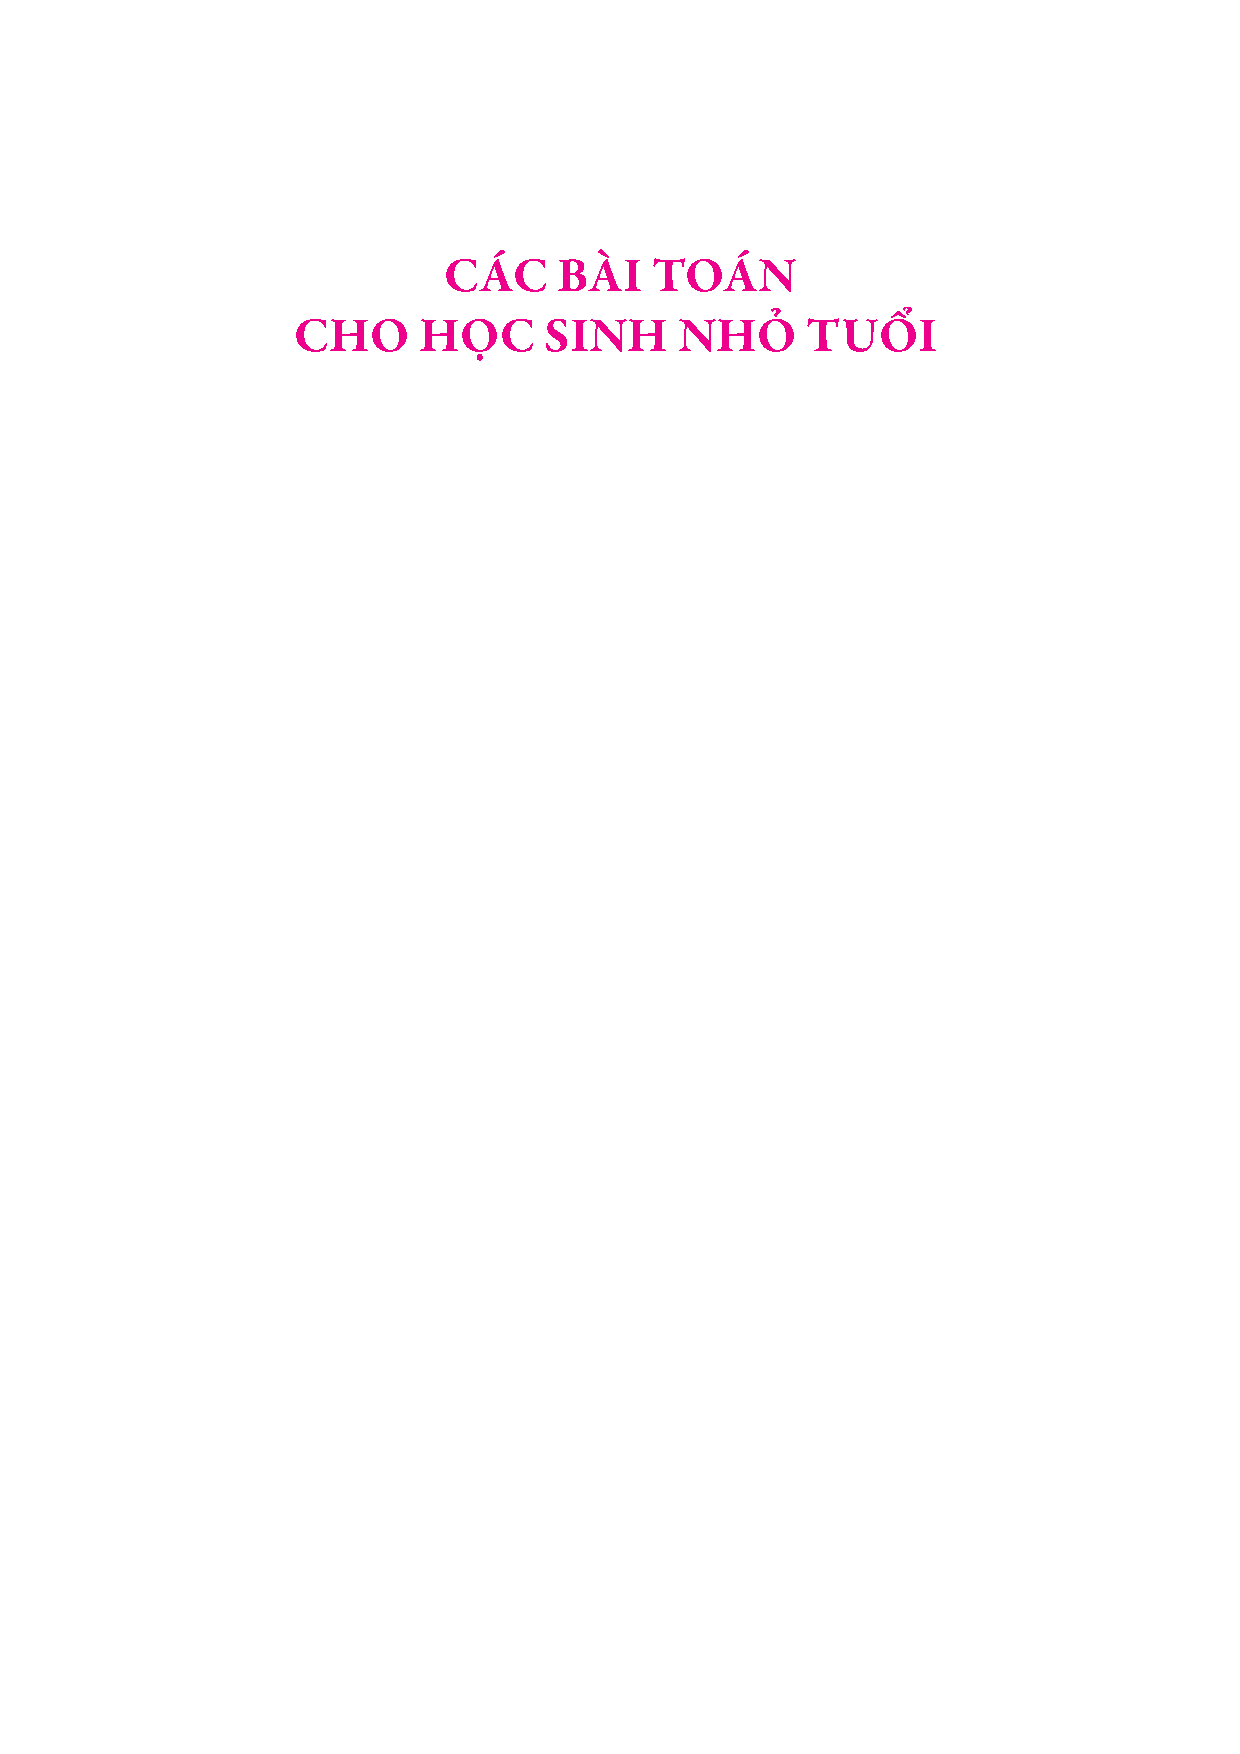
\includegraphics[scale=1]{../tieude11.pdf}}} 
\centering
\endgroup
\vspace*{33pt}

\begin{multicols}{2}
	$\pmb{1.}$	Pinocchio và Pierrot thi chạy với nhau. Pierrot chạy suốt cả quãng đường với cùng một tốc độ, còn Pinocchio chạy nhanh gấp đôi Pierrot trong nửa đầu quãng đường, và nửa sau lại chậm bằng nửa Pierrot. Hỏi ai đã thắng?
	\begin{figure}[H]
		\centering
		\vspace*{-5pt}
		\captionsetup{labelformat= empty, justification=centering}
		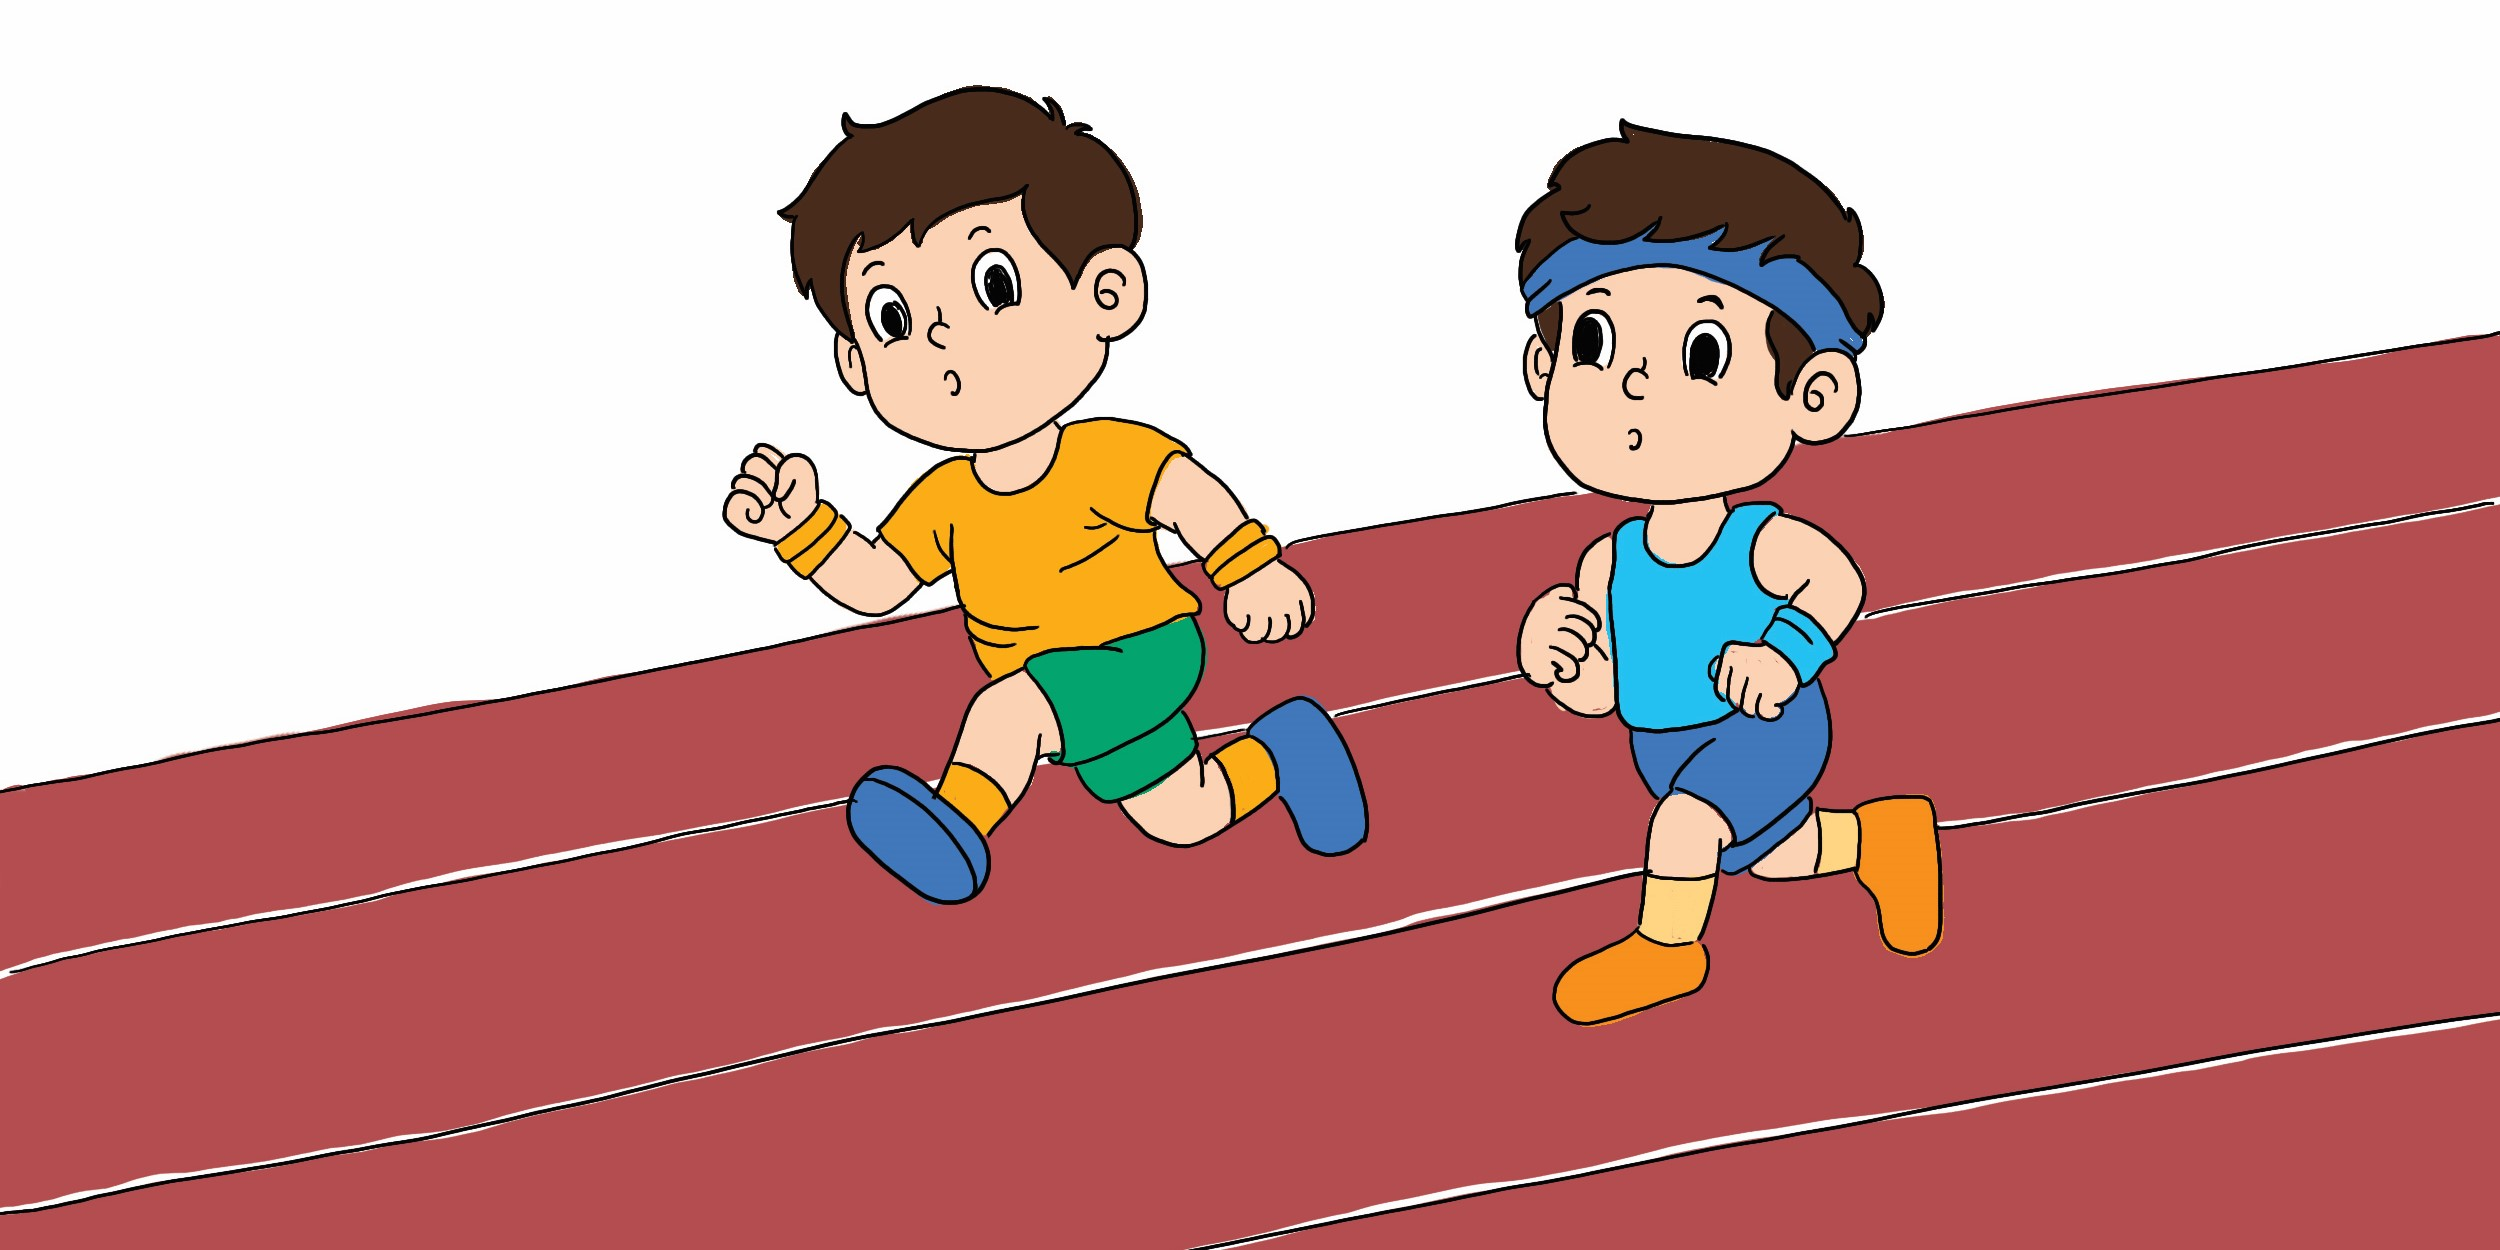
\includegraphics[width=1\linewidth]{Pi4_bai1}
		\vspace*{-15pt}
	\end{figure}
	$\pmb{2.}$ ``Còn quá sớm để các em nhìn thấy điều thần kỳ sau đây của thế giới pháp sư," cô giáo McGonagall  nói với $33$ học trò của mình ở ngôi trường Hogwarts đào tạo Phù thủy, và vung cây đũa thần ra lệnh: ``Nào, các em hãy nhắm mắt lại!" Tất cả học trò nam và một phần ba học trò nữ đều nhắm mắt phải. Tất cả học trò nữ và một phần ba các học trò nam đều nhắm mắt trái. Hỏi có bao nhiêu học trò đã nhìn thấy những gì còn quá sớm để nhìn thấy?
	\begin{figure}[H]
		\centering
		\vspace*{-10pt}
		\captionsetup{labelformat= empty, justification=centering}
		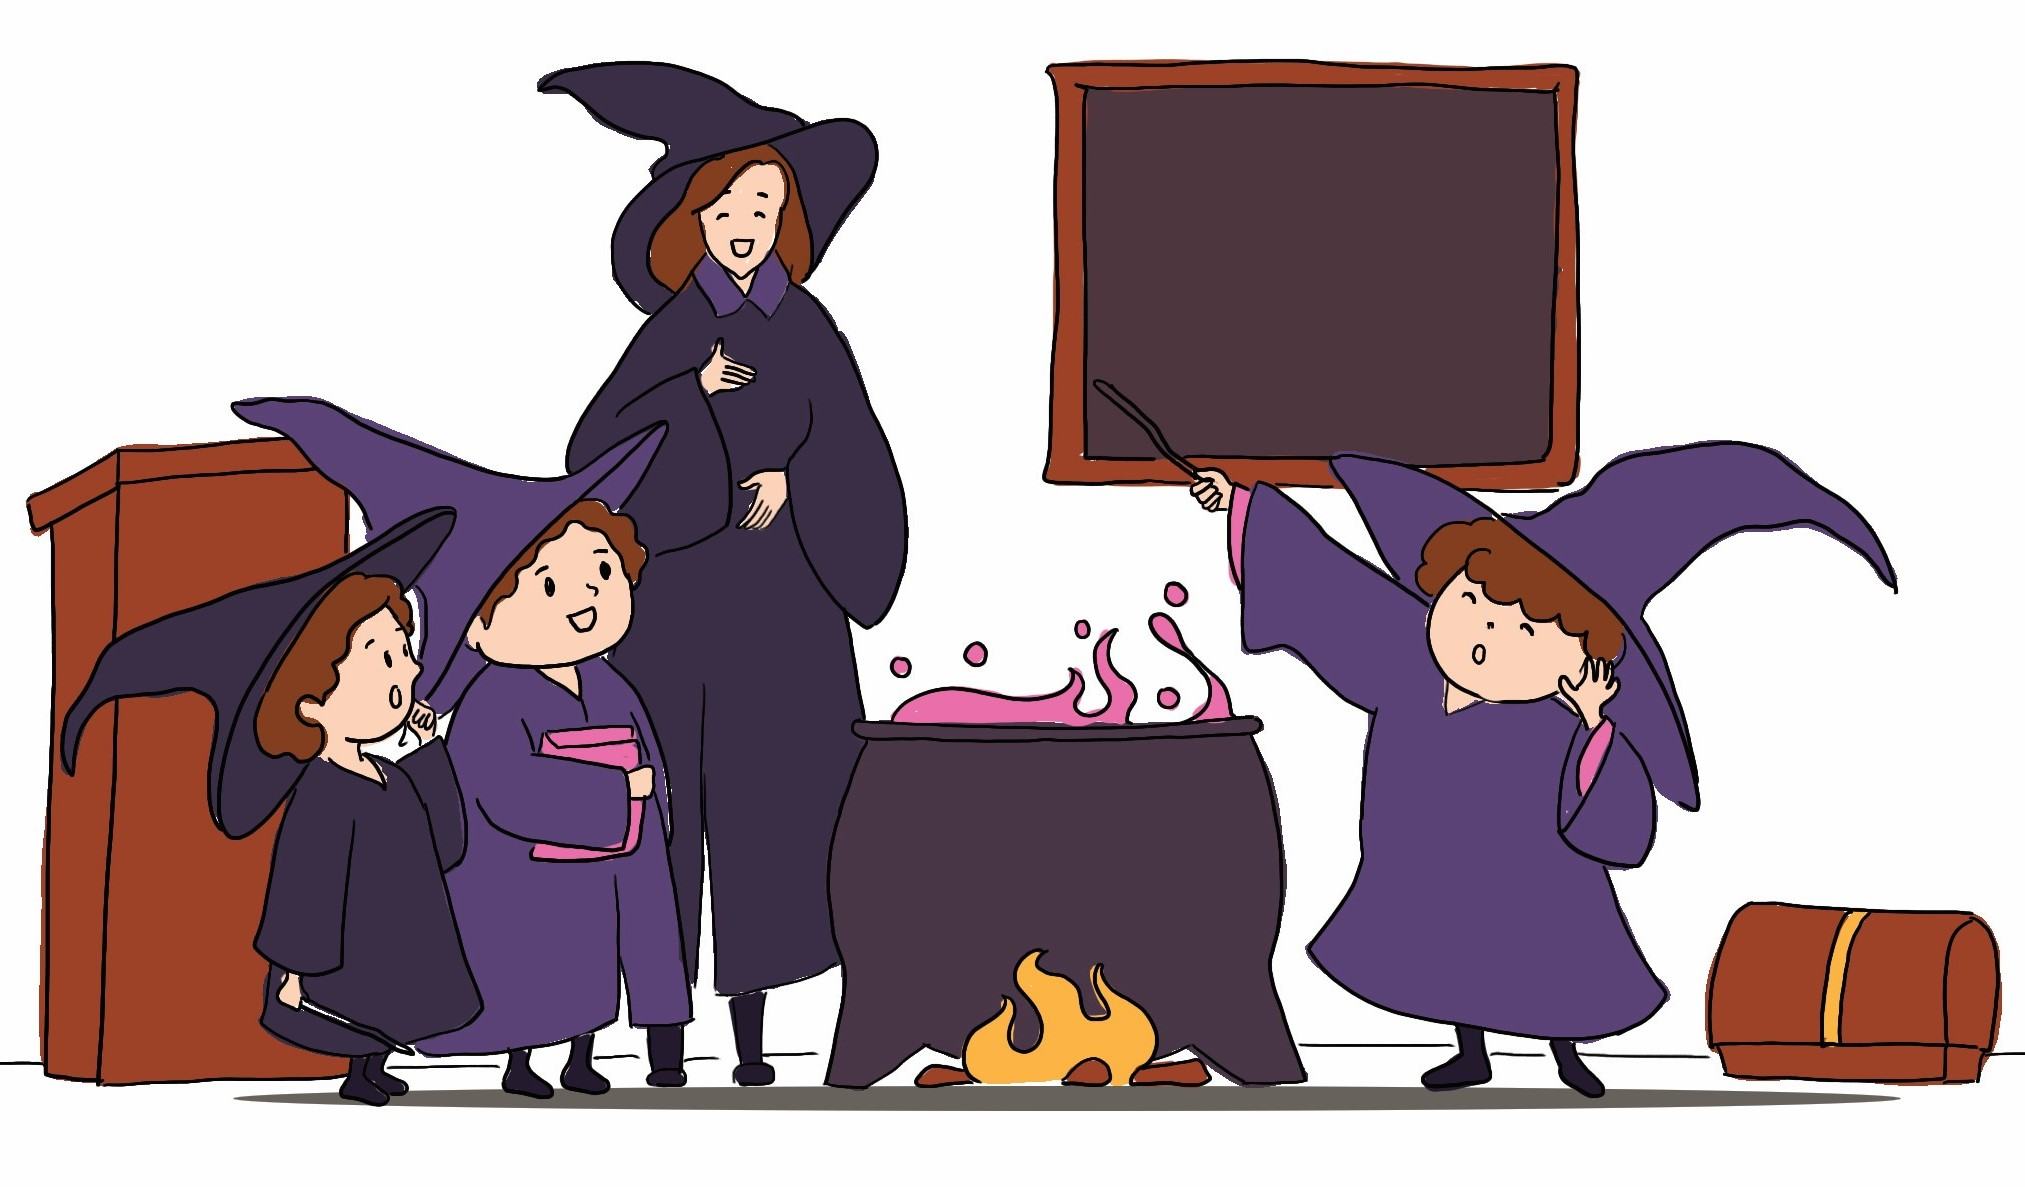
\includegraphics[width=1\linewidth]{Pi4_bai2}
		\vspace*{-15pt}
	\end{figure}
	$\pmb{3.}$ 	Bác Tư múc ra ba thìa sữa từ một ly sữa đầy và đổ chúng một ly đựng cà phê nguyên chất và khuấy đều. Sau đó bác múc ba thìa hỗn hợp thu được và đổ lại vào ly sữa. Hỏi bây giờ thứ gì nhiều hơn: cà phê trong ly đựng sữa hay sữa trong ly đựng cà phê?
	\begin{figure}[H]
		\centering
		\vspace*{5pt}
		\captionsetup{labelformat= empty, justification=centering}
		
\includegraphics[width=1\linewidth]{Pi4_bai3}
		\vspace*{-15pt}
	\end{figure}
	$\pmb{4.}$ Ma xó Brownie là một nhân vật trong văn hóa dân gian Anh và một số quốc gia khác. Đó là một dạng Phúc thần (ma thiện), tiểu yêu nghịch ngợm, thường mô tả là bé tí hon, có da nâu, ăn mặc tuềnh toàng, sinh sống gần gũi với con người, và là thần hộ mệnh cho các gia đình. Các Brownies có một xã hội thu nhỏ riêng và thường tổ chức những cuộc họp bí mật tại một tảng đá nào đó để con người không để ý tới. 
	\vskip 0.1cm
	Trong một tòa nhà bảy tầng nọ cũng có rất nhiều ma xó Brownies sinh sống. Thang máy chạy giữa tầng một và tầng cuối, dừng lại ở mỗi tầng. Ở mỗi tầng, bắt đầu từ tầng đầu tiên, có một chú Brownie bước vào thang máy, nhưng không có chú nào bước ra ngoài. Thang máy cứ di chuyển liên tục như vậy cho đến khi chú Brownie thứ một nghìn bước vào thang máy thì thang máy dừng lại. Hỏi điều này đã xảy ra ở tầng nào?
	\begin{figure}[H]
		\centering
		\vspace*{-5pt}
		\captionsetup{labelformat= empty, justification=centering}
		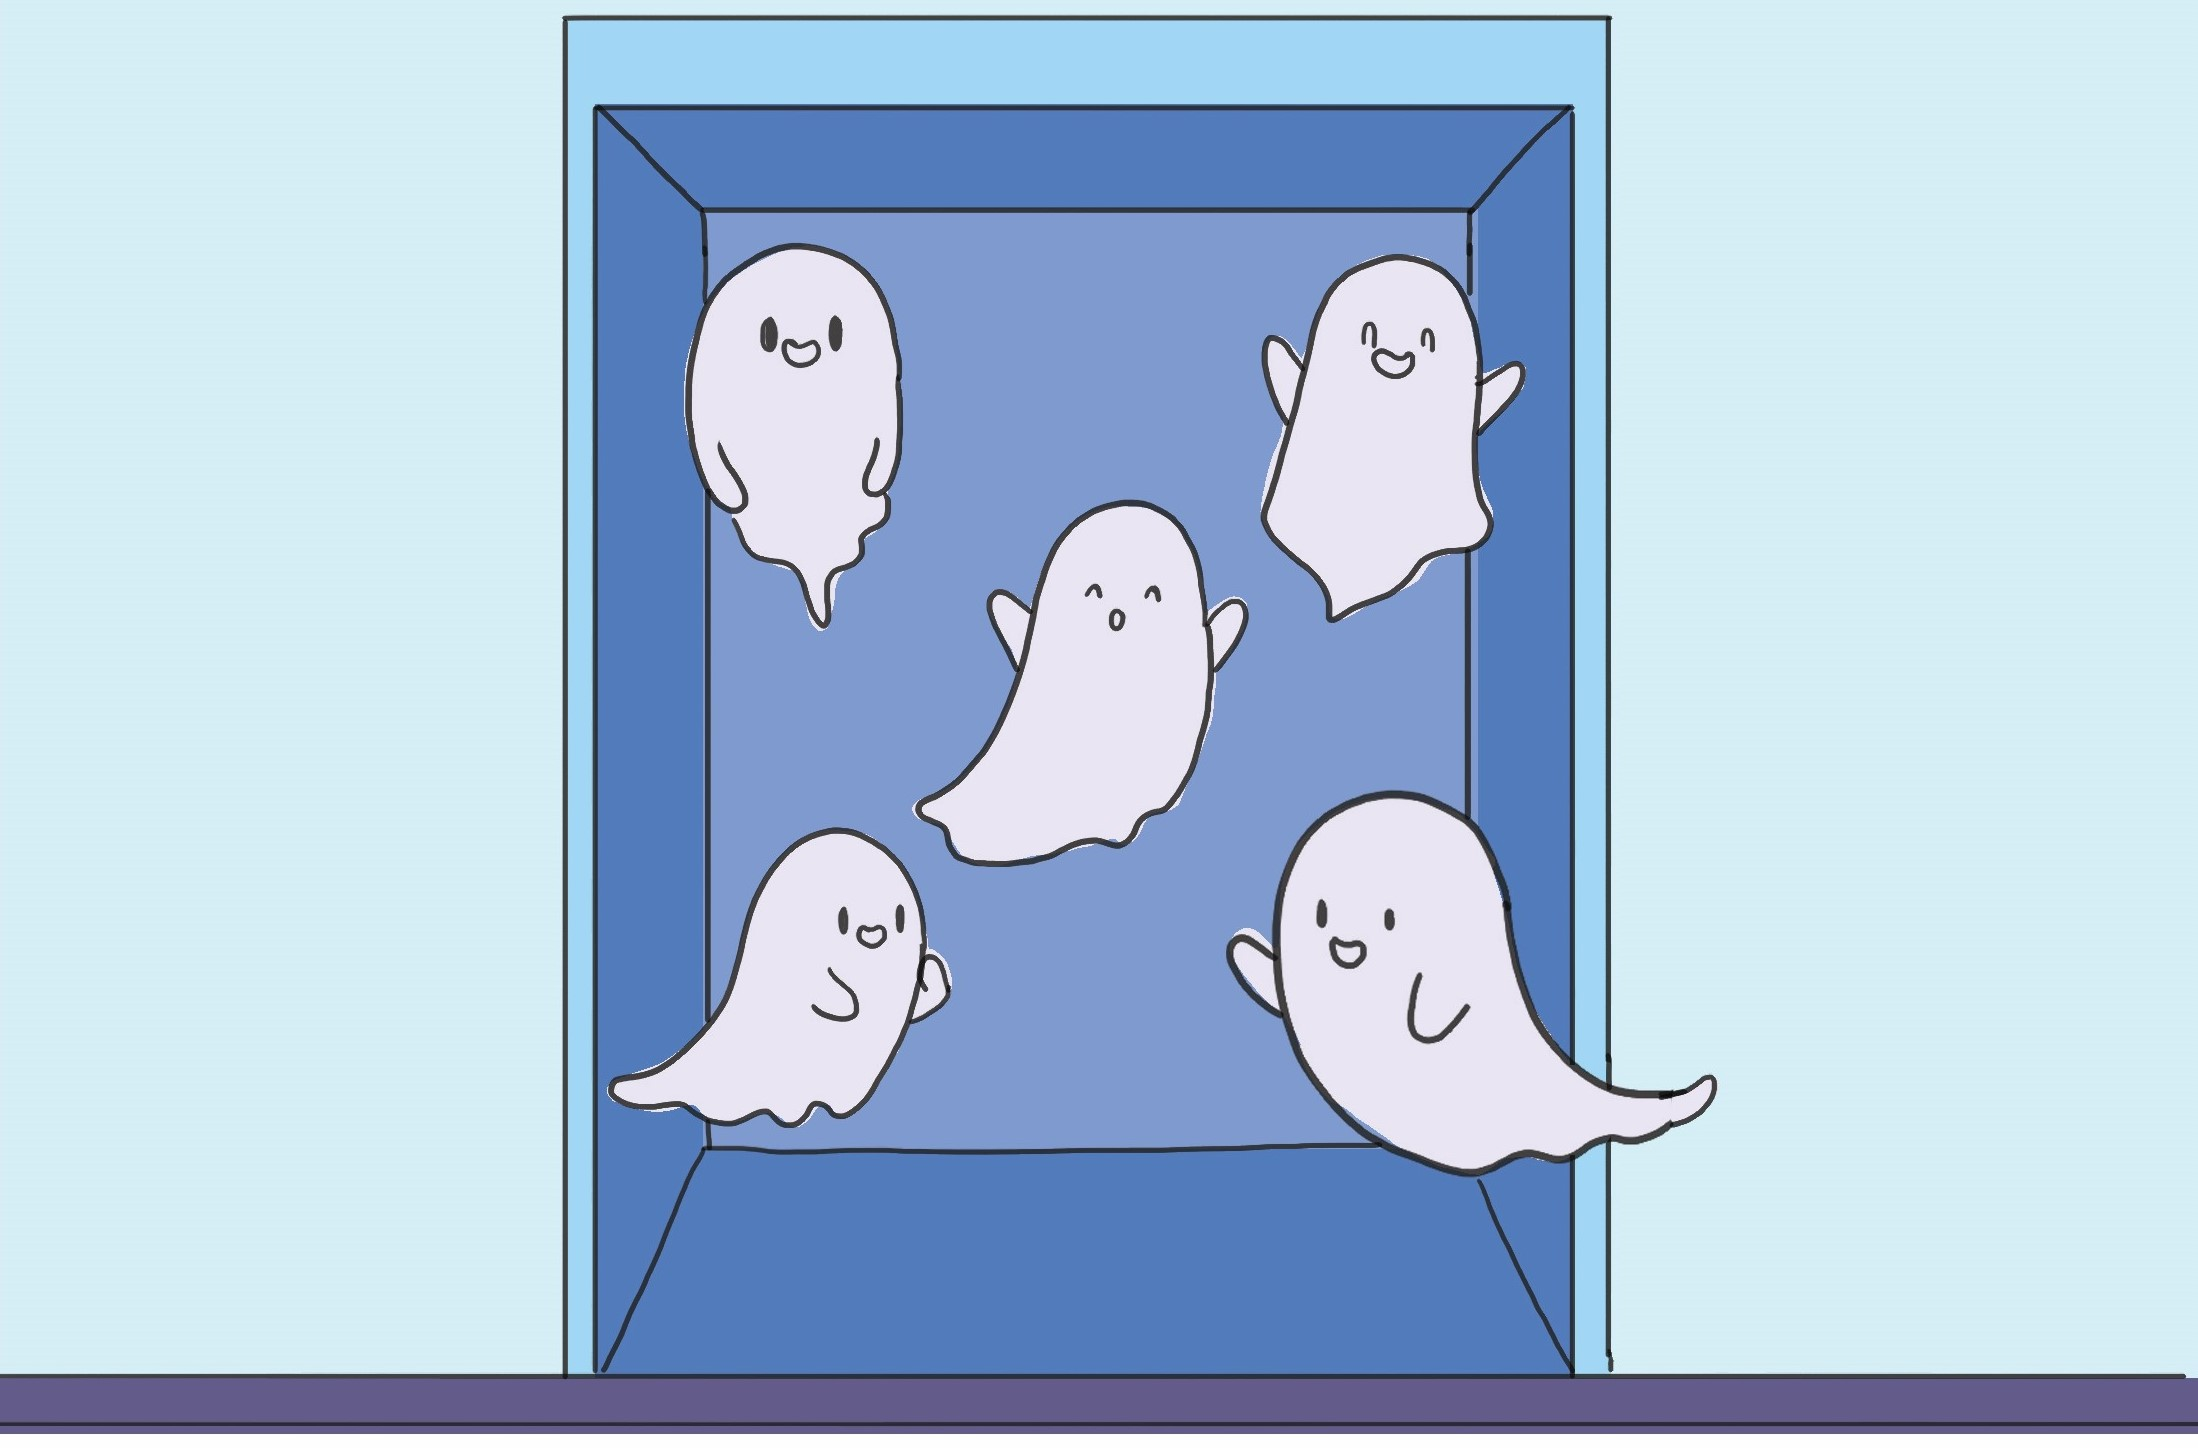
\includegraphics[width=1\linewidth]{Pi4_bai4}
		\vspace*{-15pt}
	\end{figure}
	$\pmb{5.}$ Có $40$ con thú sống trong rừng gồm cáo, sói, thỏ rừng và lửng. Hàng năm, các con thú tổ chức vũ hội hóa trang: mỗi con đeo một chiếc mặt nạ của một loài động vật khác và trong hai năm liên tiếp không con nào đeo cùng một chiếc mặt nạ của cùng một loài. Hai năm trước, có $12$ ``cáo" và $28$ ``sói" tại vũ hội, một năm trước -- có $15$ ``thỏ rừng", $10$ ``cáo" và $15$ ``lửng", và năm nay -- $15$ ``thỏ rừng" và $25$ ``cáo" . Hỏi loài thú nào có nhiều nhất trong rừng? 
	\begin{figure}[H]
		\centering
		\vspace*{-5pt}
		\captionsetup{labelformat= empty, justification=centering}
		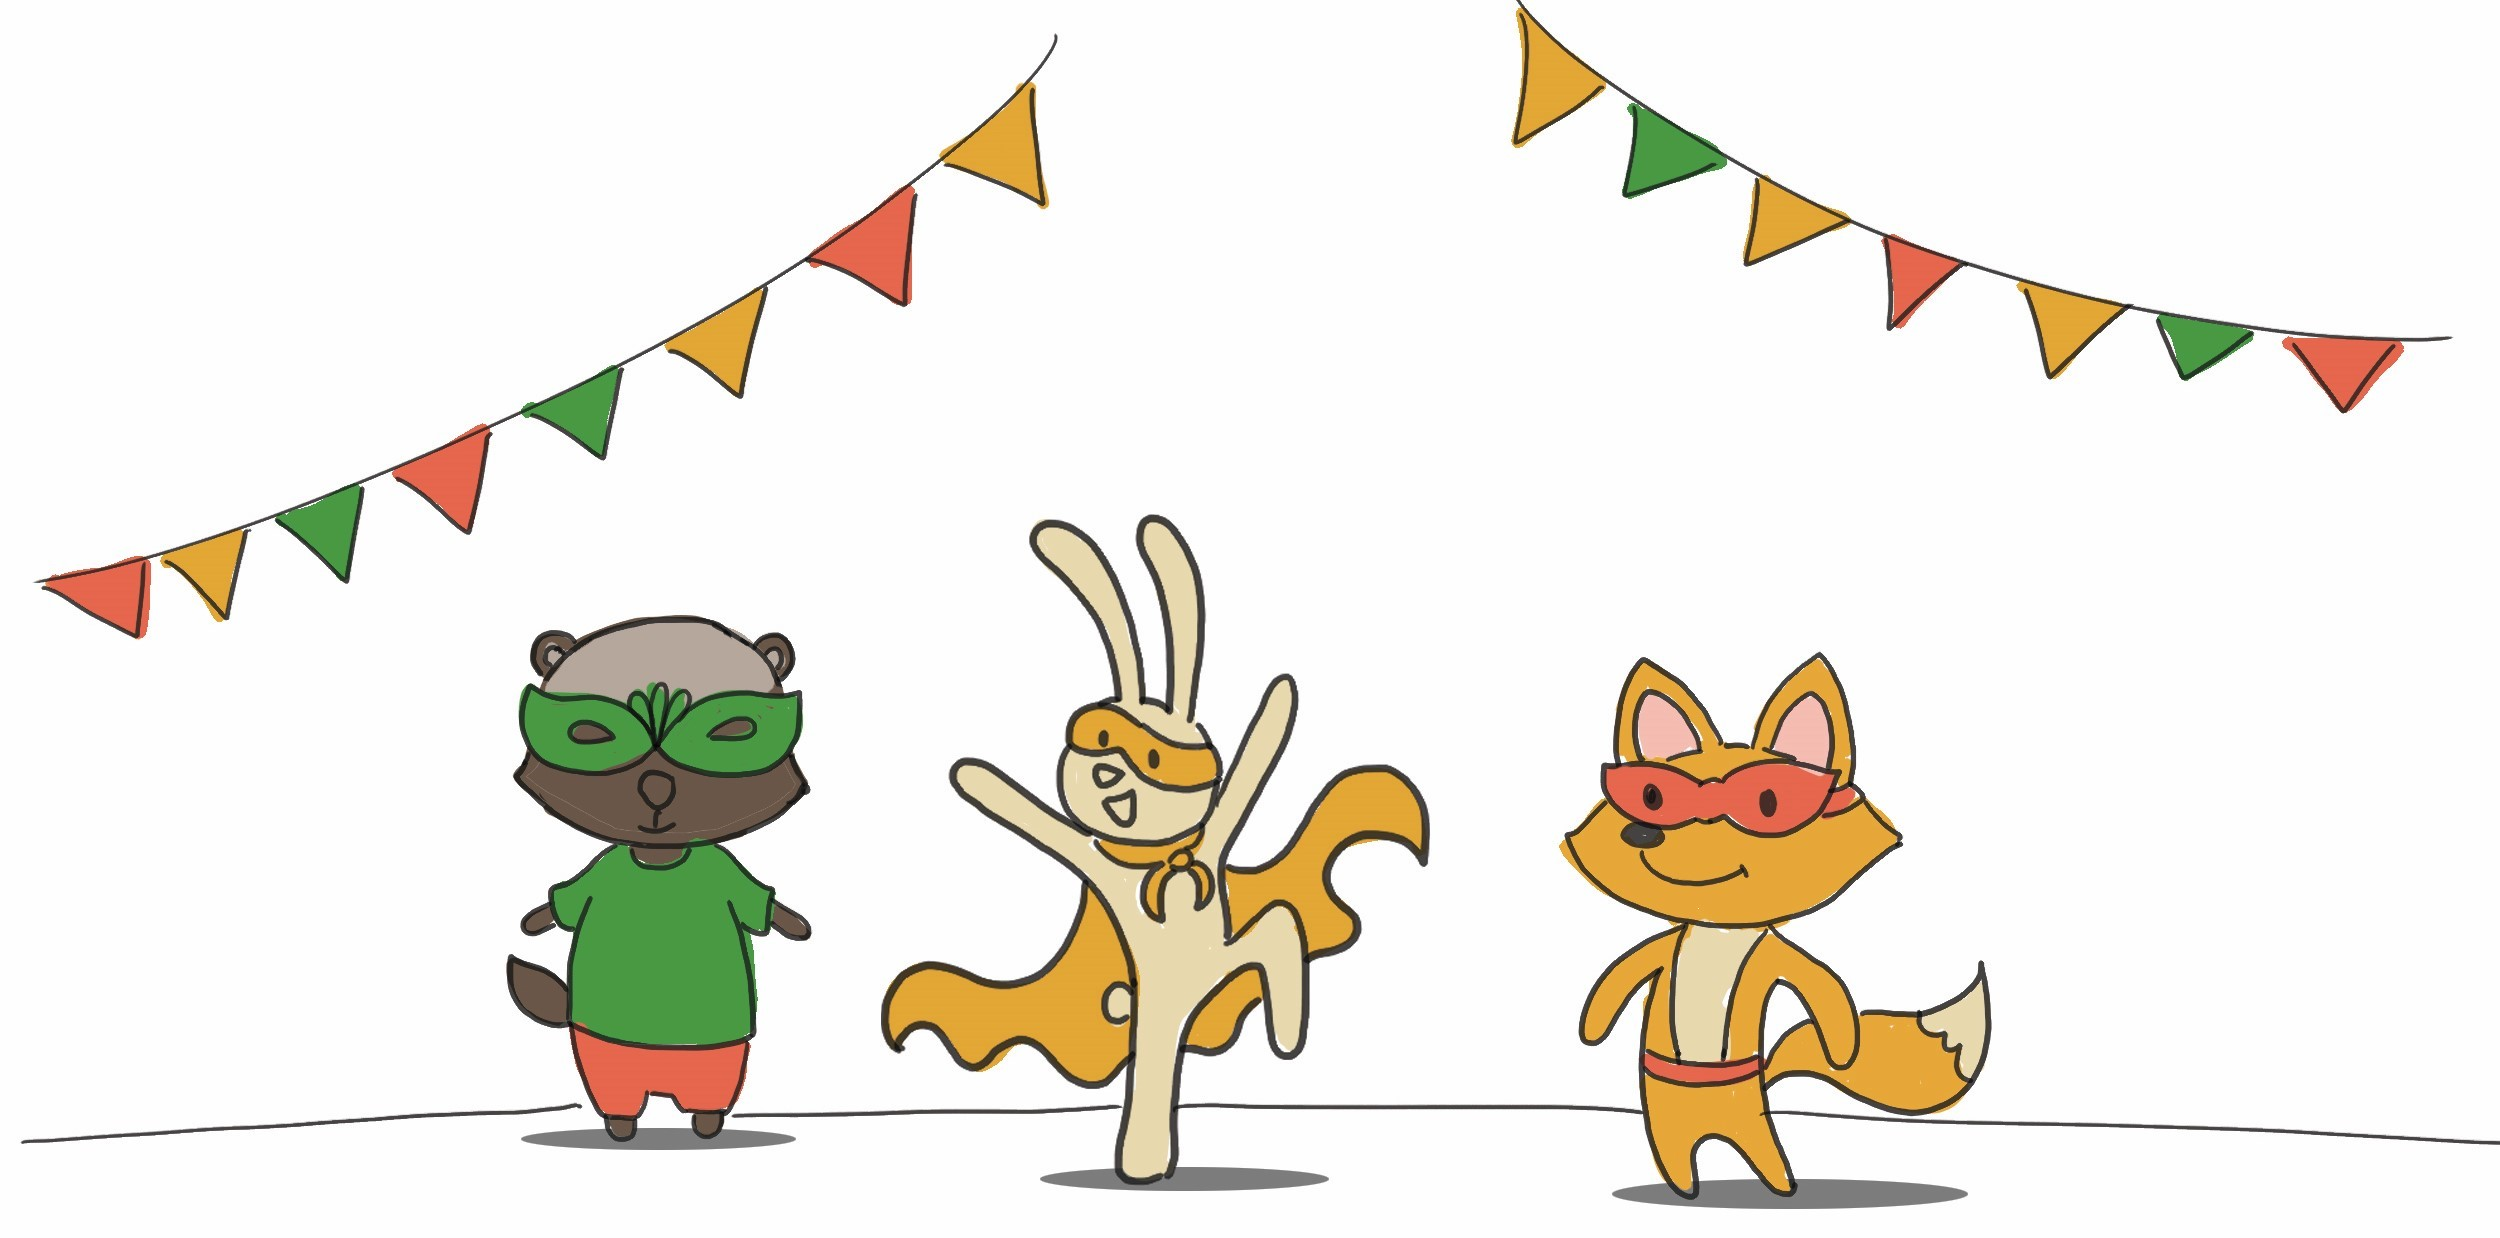
\includegraphics[width=1\linewidth]{Pi4_bai5}
		\vspace*{-15pt}
	\end{figure}
	$\pmb{6.}$ $a)$	Có tám bạn học sinh giải một đề thi gồm $8$ bài toán. Khi tổng kết lại, cô giáo thấy rằng với mỗi bài toán lại có đúng  năm bạn học sinh giải được bài đó. Chứng minh rằng có hai học sinh sao cho với mỗi bài toán trong đề có ít nhất một trong hai em giải được.
	\vskip 0.1cm
	$b)$	Em hãy chỉ ra một ví dụ rằng, nếu có đúng bốn bạn học sinh giải được mỗi bài toán, thì có thể không có hai  học sinh nào như vậy.
	\begin{figure}[H]
		\centering
		\vspace*{-5pt}
		\captionsetup{labelformat= empty, justification=centering}
		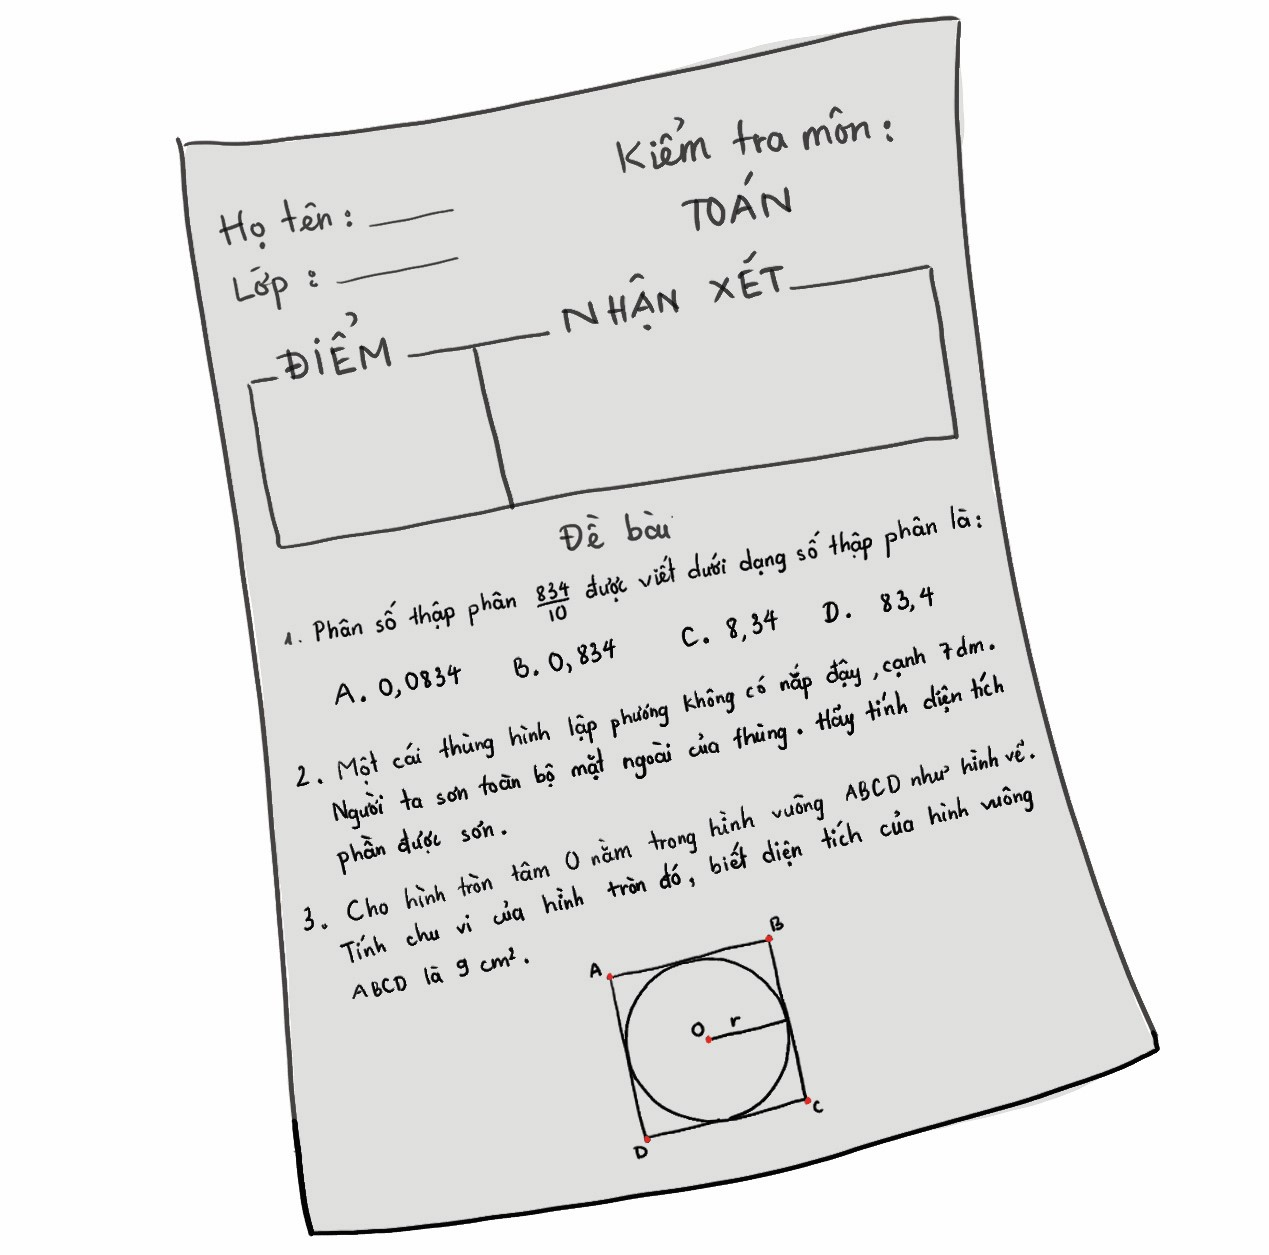
\includegraphics[width=1\linewidth]{Pi4_bai6}
		\vspace*{-15pt}
	\end{figure}
\end{multicols}
%\vspace*{-10pt}
%{\color{toancuabi}\rule{1\linewidth}{0.1pt}}
%\begingroup
%\AddToShipoutPicture*{\put(110,405){
\includegraphics[scale=1]{../tieude2.pdf}}} 
%\centering
%\endgroup
%\vspace*{75pt}
%
%\begin{multicols}{2}
%	$\pmb{1.}$ Hai anh bạn rủ nhau đi câu cá. Khi được hỏi ``Trong mỗi giỏ của các anh có bao nhiêu con cá đấy?" thì anh thứ nhất trả lời ``Trong giỏ của tôi có số cá bằng nửa số cá ở giỏ của anh kia và thêm $10$ con nữa". Anh thứ hai lại nói ``Còn trong giỏ của tôi có số cá bằng số cá trong giỏ của anh kia và thêm $20$ con nữa". Vậy cả hai anh bạn có tất cả bao nhiêu con cá nhỉ? 
%	\begin{figure}[H]
%		\centering
%		\vspace*{-10pt}
%		\captionsetup{labelformat= empty, justification=centering}
%		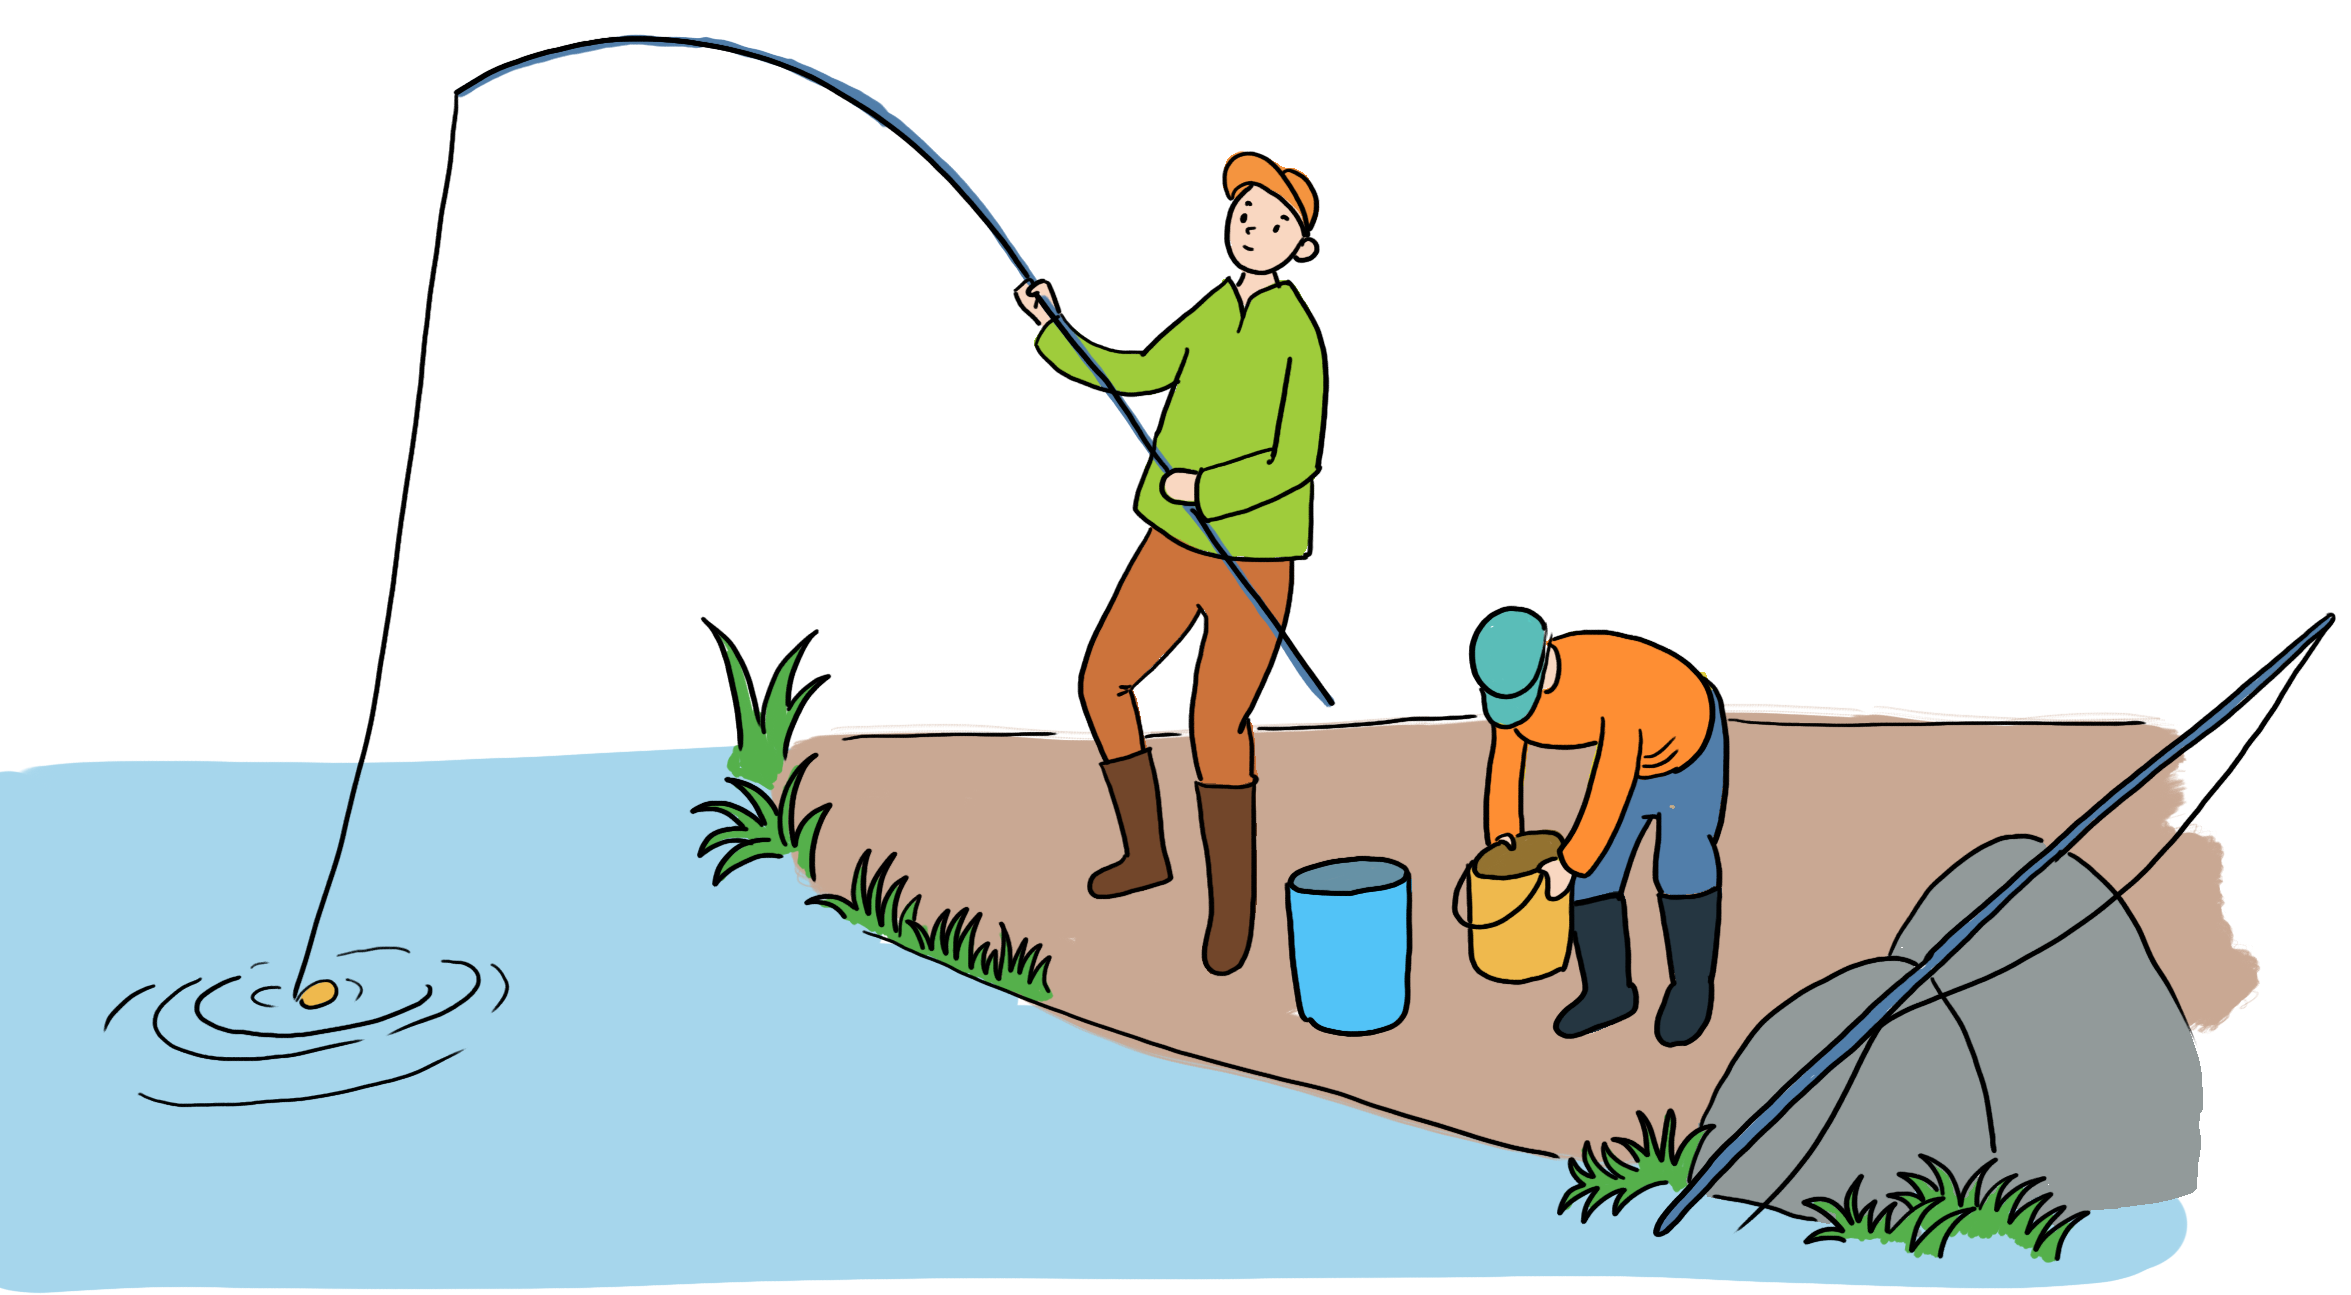
\includegraphics[width=1\linewidth]{Pi10_ToanBi_Bai1}
%		\vspace*{-15pt}
%	\end{figure}
%	\textit{Lời giải.} Một nửa số cá của anh thứ hai sẽ là nửa số cá của anh thứ nhất cộng thêm $10$ con. Vậy nửa số cá của anh thứ hai cộng thêm $10$ con sẽ bằng nửa số cá của anh thứ nhất cộng thêm $20$ con. Theo đề bài, số cá này bằng cả số cá của anh thứ nhất.
%	\vskip 0.1cm
%	Vậy một nửa số cá của anh thứ nhất là: $20$ (con)
%	\vskip 0.1cm
%	Suy ra anh thứ nhất có số cá là
%	\begin{align*}
%		2 \times 20 = 40 \text{  (con)}
%	\end{align*}
%	và anh thứ hai có số cá là 
%	\begin{align*}
%		40+20 = 60 \text{  (con).}
%	\end{align*} 
%	Tổng số cá của cả hai anh là 
%	\begin{align*}
%		40+60 = 100 \text{  (con).}
%	\end{align*}
%	Đây là bài tập đơn giản, tuy nhiên các em thử tập làm bằng nhiều cách khác nhau thông qua suy luận thông thường mà không cần dùng tới cách lập phương trình nhé.
%	\vskip 0.1cm
%	$\pmb{2.}$ Lọ lem có $100$ rổ đựng hạt dẻ, lúc đầu số hạt dẻ trong mỗi rổ là như nhau. Lọ Lem lấy đi trong rổ thứ nhất một số hạt dẻ, lấy từ rổ  thứ hai một số hạt gấp đôi như thế, lấy từ rổ thứ ba một số hạt gấp ba như thế, và cứ như vậy. Cuối cùng thì trong rổ thứ $100$ chỉ còn đúng một hạt dẻ, và còn lại ở tất cả trong $100$ rổ tổng cộng là $14950$ hạt dẻ. Hỏi ban đầu trong mỗi rổ có bao nhiêu hạt dẻ?
%	\begin{figure}[H]
%		\centering
%		\vspace*{-10pt}
%		\captionsetup{labelformat= empty, justification=centering}
%		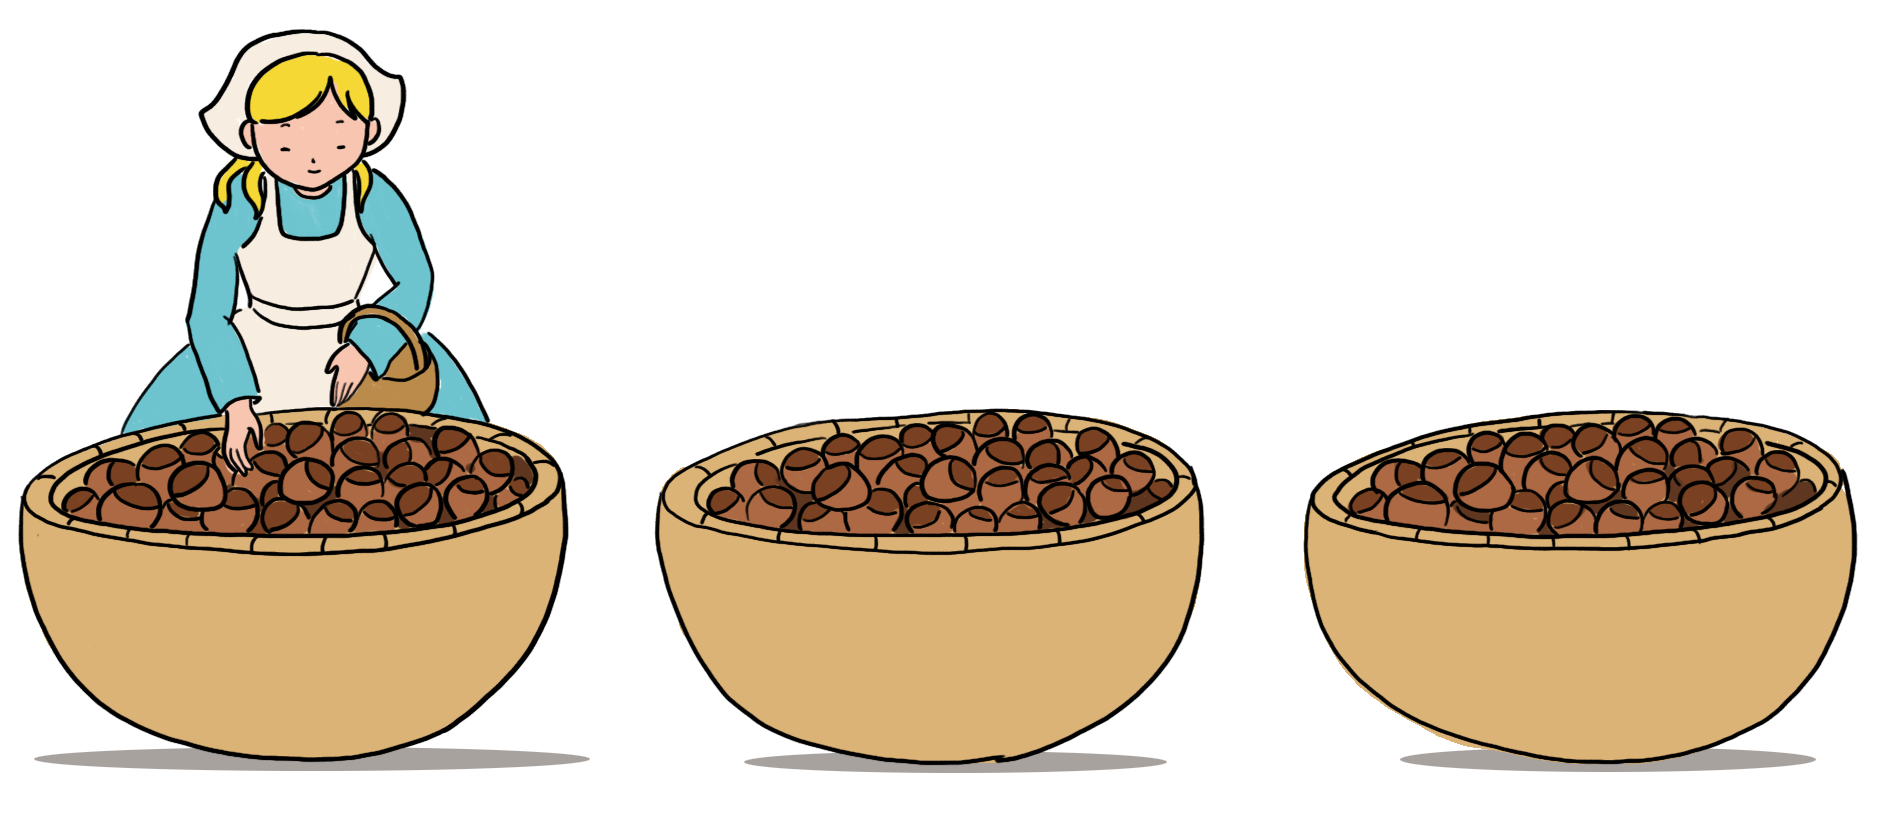
\includegraphics[width=1\linewidth]{Pi10_ToanBi_Bai2}
%		\vspace*{-15pt}
%	\end{figure}
%	\textit{Lời giải.} 	Gọi số hạt dẻ mà Lọ Lem lấy ở rổ thứ nhất là $a$, khi đó tổng cộng số hạt dẻ mà Lọ lem đã lấy đi ở $100$ rổ là
%	\begin{align*}
%		a+ 2a+\cdots+100a=5050a.
%	\end{align*} 
%	Do rổ cuối cùng còn lại $1$ hạt dẻ nên ban đầu số hạt dẻ ở rổ cuối cùng (cũng là số hạt dẻ ở các rổ khác) là: $100a+1$ (hạt).
%	\vskip 0.1cm
%	Vậy, ban đầu tổng số hạt dẻ là
%	\begin{align*}
%		100\times(100a+1) = 10000a+100 \text{  (hạt).}
%	\end{align*} 
%	Ta có hệ thức là: $10000a+100-5050 a =14950$. Từ đó suy ra $a=3$. Vì vậy ban đầu mỗi rổ có  $100\times 3+1 = 301$ hạt dẻ.
%	\vskip 0.1cm
%	$\pmb{3.}$ Hai bạn học sinh là Nam và Vũ gặp nhau tại nhà của Vũ. Nam nói ``Nếu lấy số nhà của tớ là một số có hai chữ số trừ đi số có hai chữ số tạo thành khi viết theo thứ tự ngược lại, thì sẽ ra số nhà của cậu. Vậy tớ sống ở số nhà nào?"
%	\vskip 0.1cm
%	Vũ trả lời ``Ôi, bài toán này dễ quá" -- và giải ra luôn đáp số.
%	\vskip 0.1cm
%	Vậy các bạn đó sống ở những số nhà nào nhỉ?
%	\vskip 0.1cm
%	\textit{Lời giải.} 	Nếu thực hiện phép trừ của Nam, ta sẽ nhận được số có dạng $9\times k$, ở đó $k$ là hiệu của chữ số hàng chục và chữ số hàng đơn vị. Vì số viết theo thứ tự ngược lại cũng là số có hai chữ số, nên $k\le8$. 
%	\vskip 0.1cm
%	Nếu $k<8$ thì có thể thấy có nhiều số có hai chữ số (là số nhà) mà sau khi làm phép tính trừ đã cho sẽ cho kết quả như nhau. Khi đó Vũ không thể giải được ngay câu đố của Nam. Do đó $k=8$. Các em có thể tìm thấy số nhà của Nam là $91$, và số nhà của Vũ là $72$.
%	\begin{figure}[H]
%		\centering
%		\vspace*{-5pt}
%		\captionsetup{labelformat= empty, justification=centering}
%		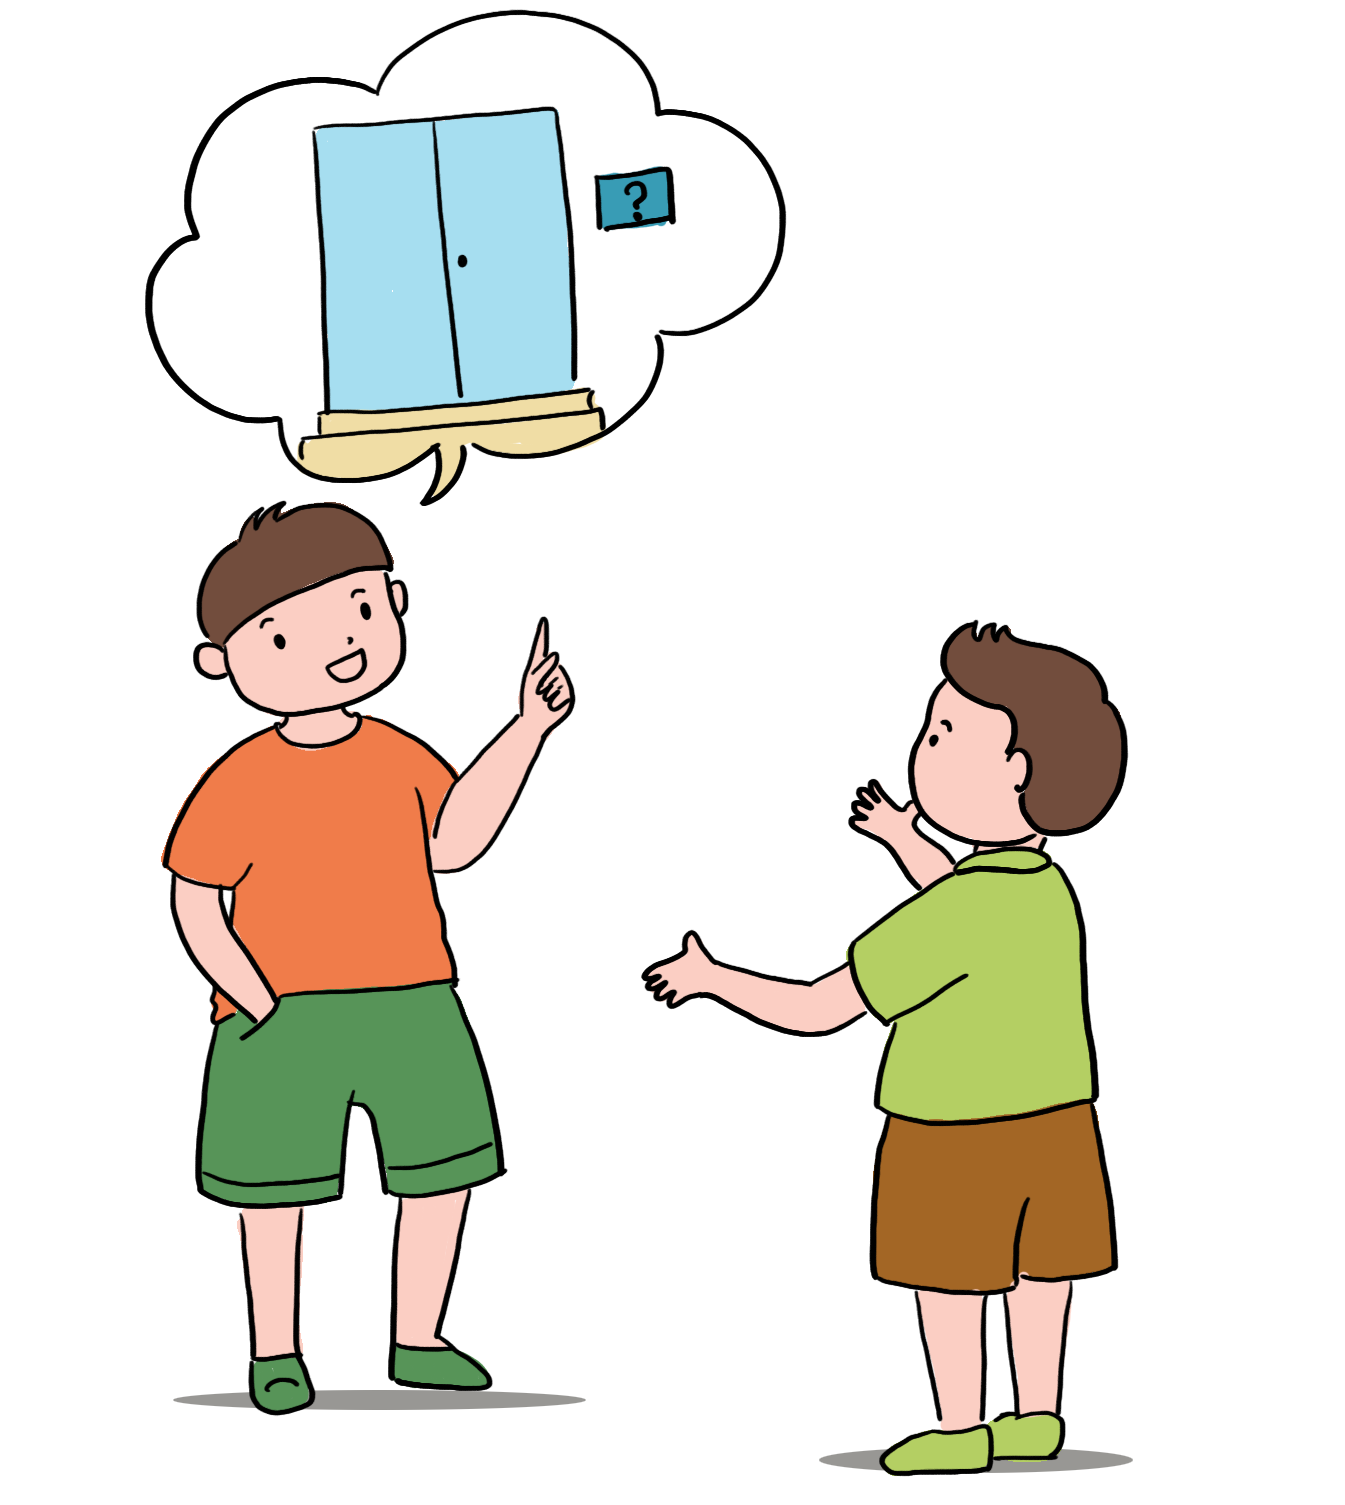
\includegraphics[width=1\linewidth]{Pi10_ToanBi_Bai3}
%		\vspace*{-15pt}
%	\end{figure}
%	$\pmb{4.}$ Lớp của Hùng có $35$ học sinh. Trong số đó có $20$ em tham gia câu lạc bộ Toán, $11$ em tham gia câu lạc bộ Khéo tay, $10$ em không tham gia vào hai nhóm này. Hỏi có tất cả bao nhiêu em vừa tham gia CLB Toán lại vẫn không quên tham gia cả CLB Khéo tay nhỉ?
%	\begin{figure}[H]
%		\centering
%		\vspace*{-5pt}
%		\captionsetup{labelformat= empty, justification=centering}
%		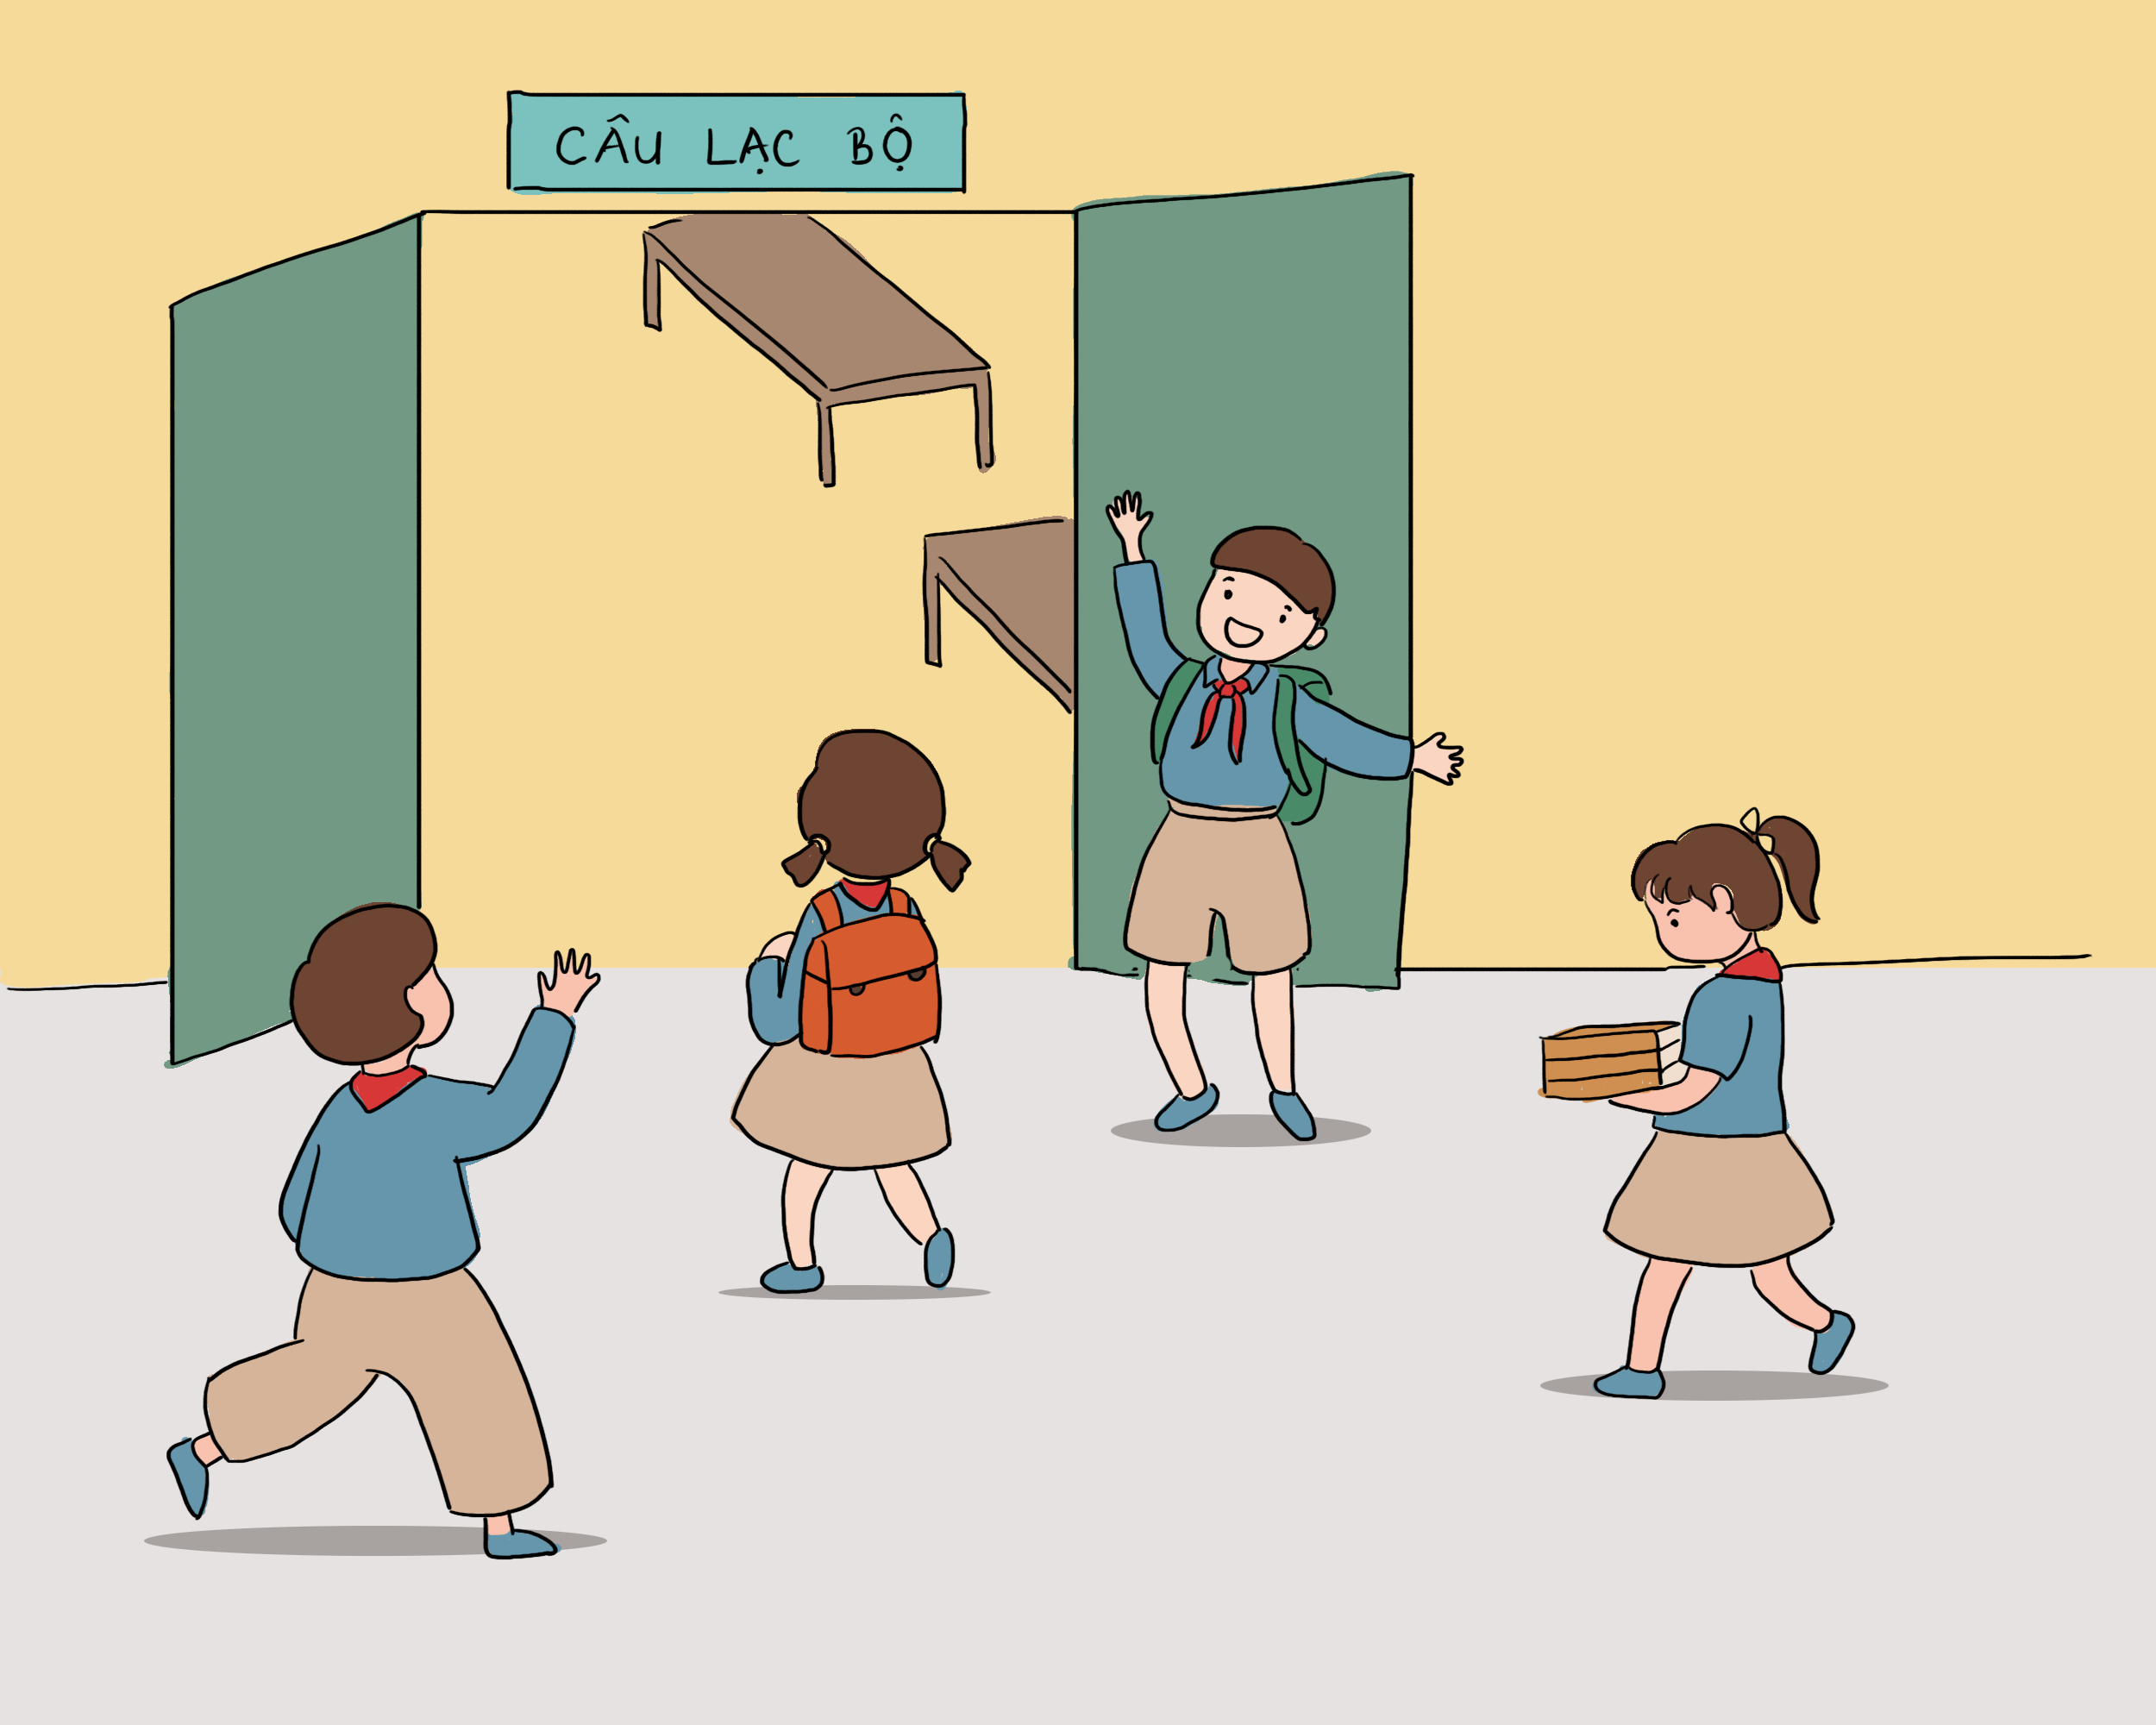
\includegraphics[width=1\linewidth]{Pi10_ToanBi_Bai4}
%		\vspace*{-15pt}
%	\end{figure}
%	\textit{Lời giải.} 	Chúng ta chia toàn bộ số học sinh trong lớp thành bốn danh sách, mà không có em nào ở trong hai danh sách khác nhau, như sau. Danh sách ``toán thuần tuý" gồm các bạn chỉ tham gia CLB Toán, danh sách ``khéo tay thuần tuý" gồm các bạn chỉ tham gia CLB Khéo tay, danh sách ``giỏi toán lại khéo tay" gồm các bạn tham gia cả $2$ CLB  và cuối cùng là danh sách ``rảnh rỗi" là các bạn không tham gia vào hai CLB này. Theo đề bài, danh sách ``rảnh rỗi" có $10$ bạn, vì thế có $25$ bạn không ``rảnh rỗi". Trong số $25$ bạn này có $20$ bạn tham gia nhóm Toán, vì thế số ``khéo tay thuần tuý" là $5$ bạn. Vậy số bạn vừa tham gia nhóm Toán lại ``khéo tay" nữa là 
%	\begin{align*}
%		11-5 = 6 \text{ (bạn).}
%	\end{align*}
%	$\pmb{5.}$ Tùng đến trường mới có nhiều chuyện rất vui nên về khoe với bạn bè.
%	\begin{figure}[H]
%		\centering
%		%		\vspace*{5pt}
%		\captionsetup{labelformat= empty, justification=centering}
%		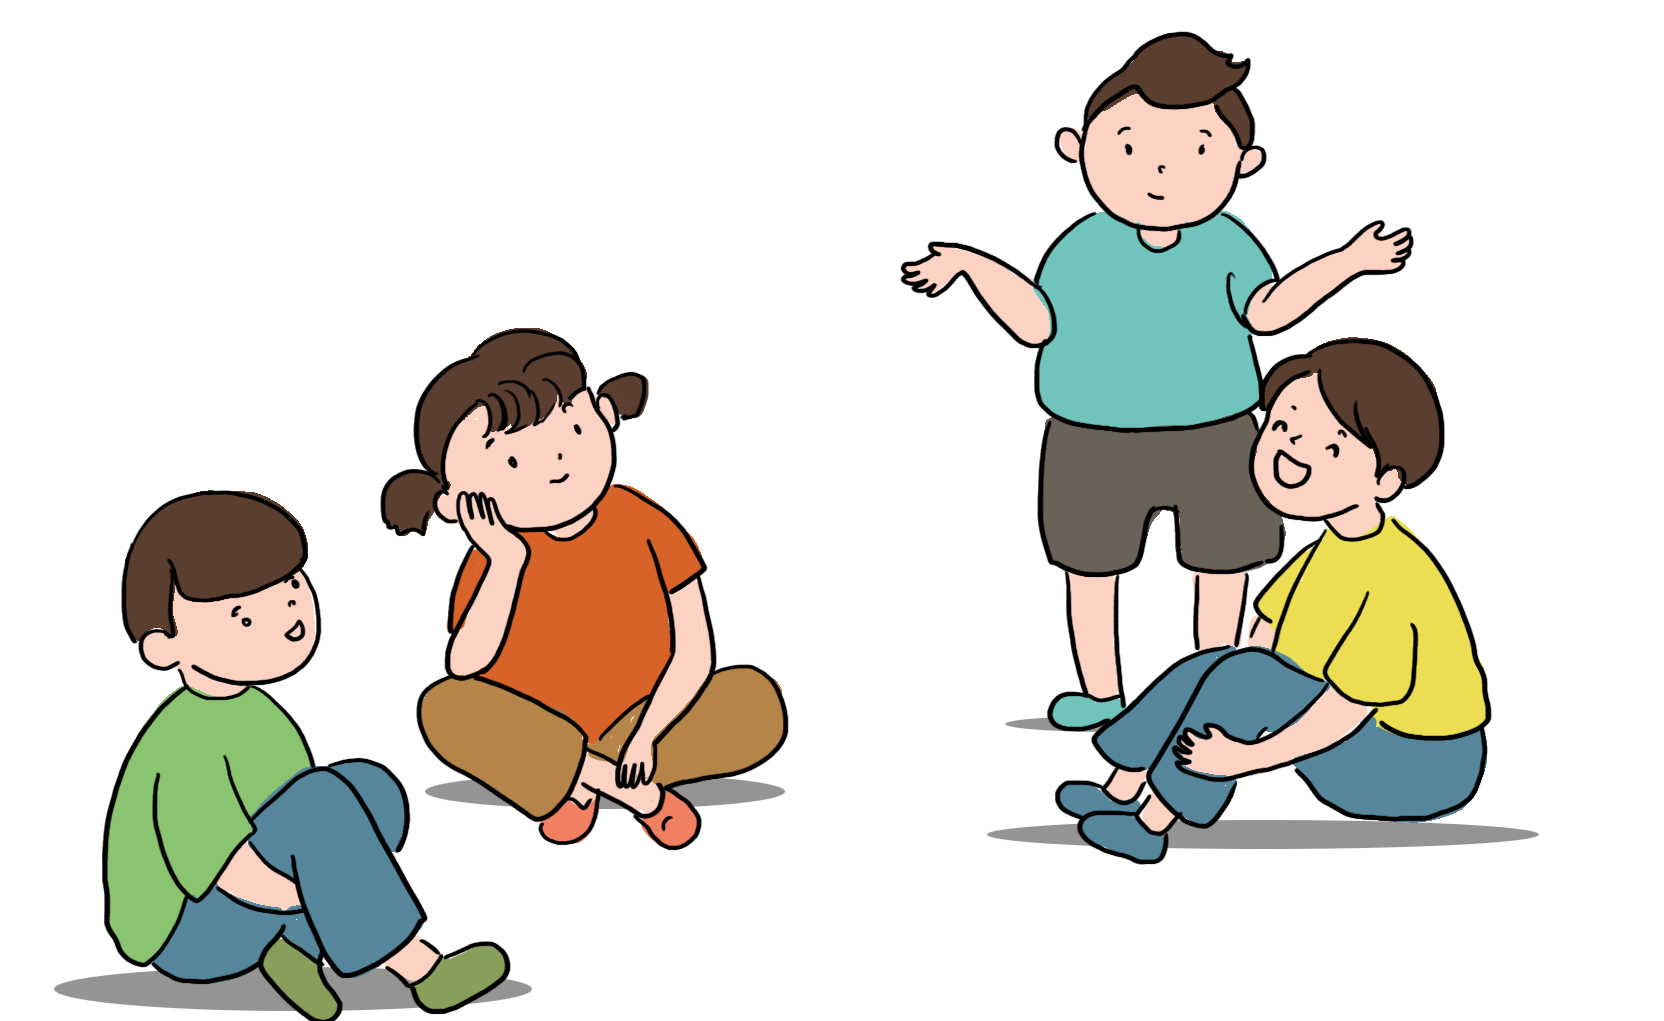
\includegraphics[width=1\linewidth]{Pi10_ToanBi_Bai5}
%		\vspace*{-15pt}
%	\end{figure}
%	-- Lớp tớ có $35$ học sinh. Và các cậu có tưởng tượng được không, mỗi người lại kết bạn với đúng $11$ học sinh cùng lớp.
%	\vskip 0.1cm
%	-- Không thể thế được! Bách, người bạn thân của Tùng vừa đạt giải trong một cuộc thi Olympic, ngay lập tức trả lời.
%	\vskip 0.1cm
%	Vì sao Bách lại nghĩ như vậy nhỉ?
%	\vskip 0.1cm
%	\textit{Lời giải.} 	Ta biểu diễn mỗi học sinh bằng một điểm trên mặt phẳng. Nếu hai học sinh kết bạn với nhau ta sẽ nối hai điểm tương ứng bởi một đoạn thẳng. Như vậy có $35$ điểm, mỗi điểm được nối đúng với $11$ điểm khác. Khi đó tổng số các đầu của các đoạn thẳng nối quan hệ bạn bè là $35\times11$ là một số lẻ. Điều này là vô lý do mỗi đoạn thẳng thể hiện quan hệ bạn bè có đúng hai điểm đầu mút. 
%	\vskip 0.1cm
%	$\pmb{6.}$ Có $55$ em học sinh tham gia một cuộc thi Olympic. Tất cả các em đều nộp bài. Khi chấm bài, mỗi câu hỏi được chấm bởi một trong ba loại điểm: điểm ``$+$" nếu câu hỏi được trả lời hoàn toàn đúng; điểm ``$-$" nếu câu hỏi đã có trả lời nhưng chưa ra đúng đáp số; và điểm ``$0$" nếu câu hỏi chưa được trả lời. Sau khi chấm toàn bộ bài thi, ban tổ chức thấy không có hai bài thi nào có cả các số điểm ``$+$" và số điểm ``$-$" đồng thời trùng nhau. Vậy trong kỳ thi Olympic đó phải có ít nhất bao nhiêu câu hỏi?
%	\vskip 0.1cm
%	\textit{Lời giải.} 	Giả sử $a$ là số câu hỏi được ra.  Ta chia ra các trường hợp sau
%	\vskip 0.1cm
%	$1.$ Bài thi có tất cả các câu hỏi đều được trả lời: Khi đó số các bài thi sẽ không vượt quá $a+1$ bài: từ bài có $a$ dâú ``$+$" và $0$ dấu ``$-$" cho đến bài có $0$ dấu ``$+$" và $a$ dấu ``$-$".  
%	\vskip 0.1cm
%	Bài thi trong đó chỉ có đúng một bài chưa có trả lời (có một điểm ``$0$"): Số các bài thi  nhiều nhất là $a$ bài (từ $a-1$ điểm ``$+$" và $0$ điểm ``$-$" cho đến bài có $0$ điểm ``$+$" và $a-1$ điểm ``$-$"). $\ldots$
%	\vskip 0.1cm
%	Và cứ xét như vậy, ta thấy tổng số các bài thi nhiều nhất là 
%	\begin{align*}
%		(a\!+\!1)\!+\!a\!+\!(a\!-\!1)\!+\!\cdots\!+\!1=\dfrac{(a\!+\!1)(a\!+\!2)}{2}.
%	\end{align*}
%	Từ đó ta có $55\le\dfrac{(a+1)(a+2)}{2}$. Với $a=9$ ta có $\dfrac{10\cdot11}{2}=55$. Vậy là $a \ge 9$. 
%	\vskip 0.1cm
%	Vì vậy số câu hỏi ít nhất được ra là $9$ câu.
%\end{multicols}
\newpage
\begingroup
\thispagestyle{toancuabinone}
\blfootnote{$^1$\color{toancuabi}Ottawa, Canada.}
\AddToShipoutPicture*{\put(60,733){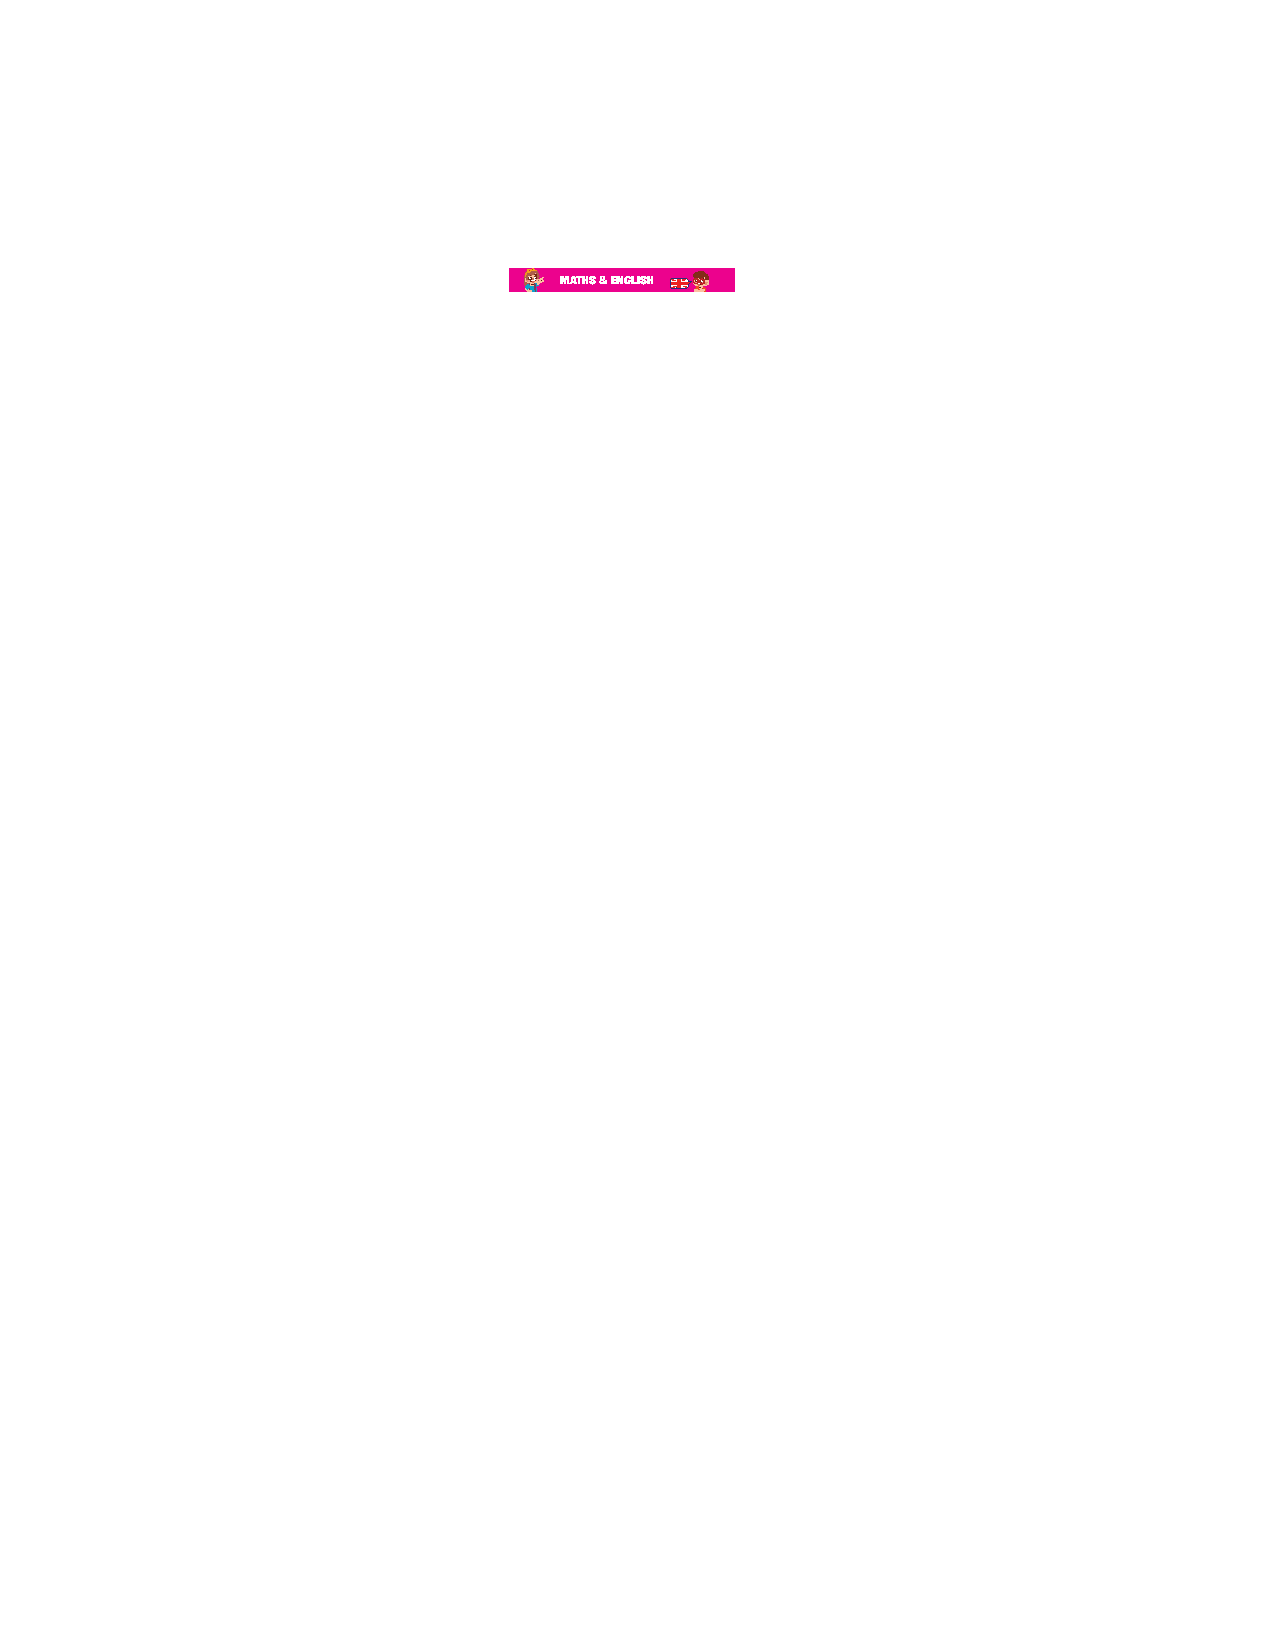
\includegraphics[width=17.2cm]{../mathc.pdf}}}
%\AddToShipoutPicture*{\put(-2,733){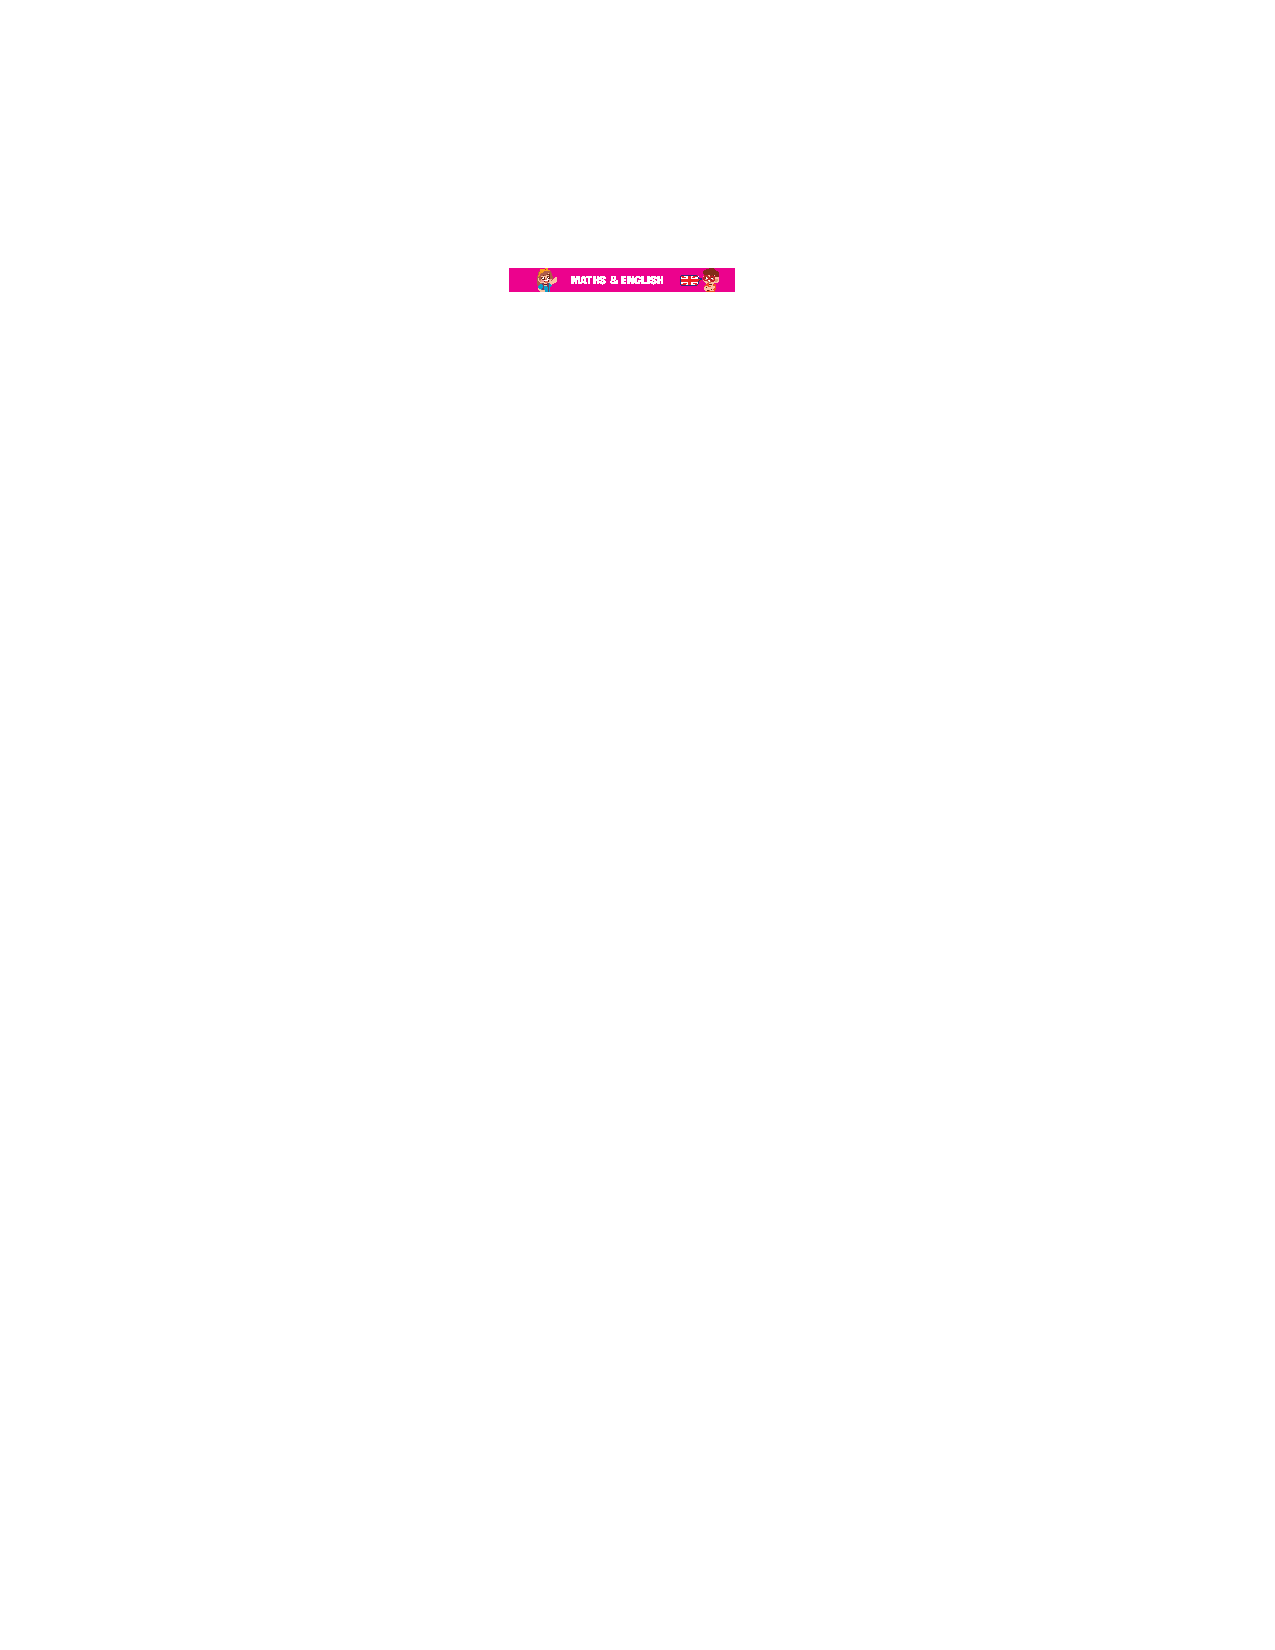
\includegraphics[width=17.2cm]{../mathl.pdf}}} 
\AddToShipoutPicture*{\put(145,680){
\includegraphics[scale=1]{../tieude3.pdf}}} 
\centering
\endgroup
\vspace*{25pt}

\begin{multicols}{2}
		In this article, we discuss some applications of pattern recognition in graph theory.
	\vskip 0.2cm
	\PIbox{
		{\color{toancuabi}\textbf{Example} (Match the phrases)\textbf{.}} Match the phrases in Vietnamese on the left of the table below,
		with their translations into English on the right of the table.}
	\begin{table}[H]
		\vspace*{-5pt}
		\centering
		\captionsetup{labelformat= empty, justification=centering}
		\renewcommand{\arraystretch}{1.2}
		\setlength{\tabcolsep}{4pt}
		\resizebox{\columnwidth}{!}{\begin{tabular}{|c|l|c|c|l|}
				\cline{1-2} \cline{4-5}
				\multirow{ 2}{*}{$1$}  & \multirow{ 2}{*}{băng}       &  & \multirow{ 2}{*}{A} & bouquet (a bunch        \\
				&      &  & &of flowers)        \\
				\cline{1-2} \cline{4-5} 
				$2$  & bó         &  & B & chalk                               \\ \cline{1-2} \cline{4-5} 
				$3$  & bó hoa     &  & C & circle                              \\ \cline{1-2} \cline{4-5} 
				$4$  & cánh hoa   &  & D & cluster                              \\ \cline{1-2} \cline{4-5} 
				$5$  & đá         &  & E & detour                              \\ \cline{1-2} \cline{4-5} 
				$6$  & đá lửa     &  & F & fire                                \\ \cline{1-2} \cline{4-5} 
				\multirow{ 2}{*}{$7$}  & \multirow{ 2}{*}{đá phấn}    &  & \multirow{ 2}{*}{G} & flint (a stone used \\
				&     &  &  & to make sparks) \\
				\cline{1-2} \cline{4-5} 
				$8$  & đường      &  & H & flower                              \\ \cline{1-2} \cline{4-5} 
				$9$  & đường vòng &  & I & ice                                 \\ \cline{1-2} \cline{4-5} 
				$10$ & hoa        &  & J & iceberg                             \\ \cline{1-2} \cline{4-5} 
				$11$ & lửa        &  & K & mountain                            \\ \cline{1-2} \cline{4-5} 
				$12$ & mở         &  & L & petal                               \\ \cline{1-2} \cline{4-5} 
				$13$ & mở đường   &  & M & pollen                              \\ \cline{1-2} \cline{4-5} 
				$14$ & mở mắt     &  & N & powder                              \\ \cline{1-2} \cline{4-5} 
				$15$ & núi        &  & O & road                                \\ \cline{1-2} \cline{4-5} 
				$16$ & núi băng   &  & P & rock                                \\ \cline{1-2} \cline{4-5} 
				$17$ & núi lửa    &  & Q & tear (as in teardrop)               \\ \cline{1-2} \cline{4-5} 
				$18$ & nước đá    &  & R & to make aware                       \\ \cline{1-2} \cline{4-5} 
				$19$ & nước mắt   &  & S & to open                             \\ \cline{1-2} \cline{4-5} 
				$20$ & phấn       &  & T & to pave the way                     \\ \cline{1-2} \cline{4-5} 
				$21$ & phấn hoa   &  & U & volcano                             \\ \cline{1-2} \cline{4-5} 
				$22$ & vòng       &  & V & wreath                              \\ \cline{1-2} \cline{4-5} 
				$23$ & vòng hoa   &  &   &                                     \\ \cline{1-2} \cline{4-5} 
		\end{tabular}}
		\vspace*{-10pt}
	\end{table}
\textit{Solution.}
We use a graph theory approach from the point of view of an English speaker to solve the problem.
\vskip 0.1cm
First, we look at the Vietnamese phrases. They are single- and double--word phrases.
We connect the phrases in a graph so that each pair of phrases consists of a single--word phrases and a double-word phrase,
the double--word phrase basically contains the single-word phrase. See the diagram below.
\begin{figure}[H]
	\vspace*{-5pt}
	\centering
	\captionsetup{labelformat= empty, justification=centering}
	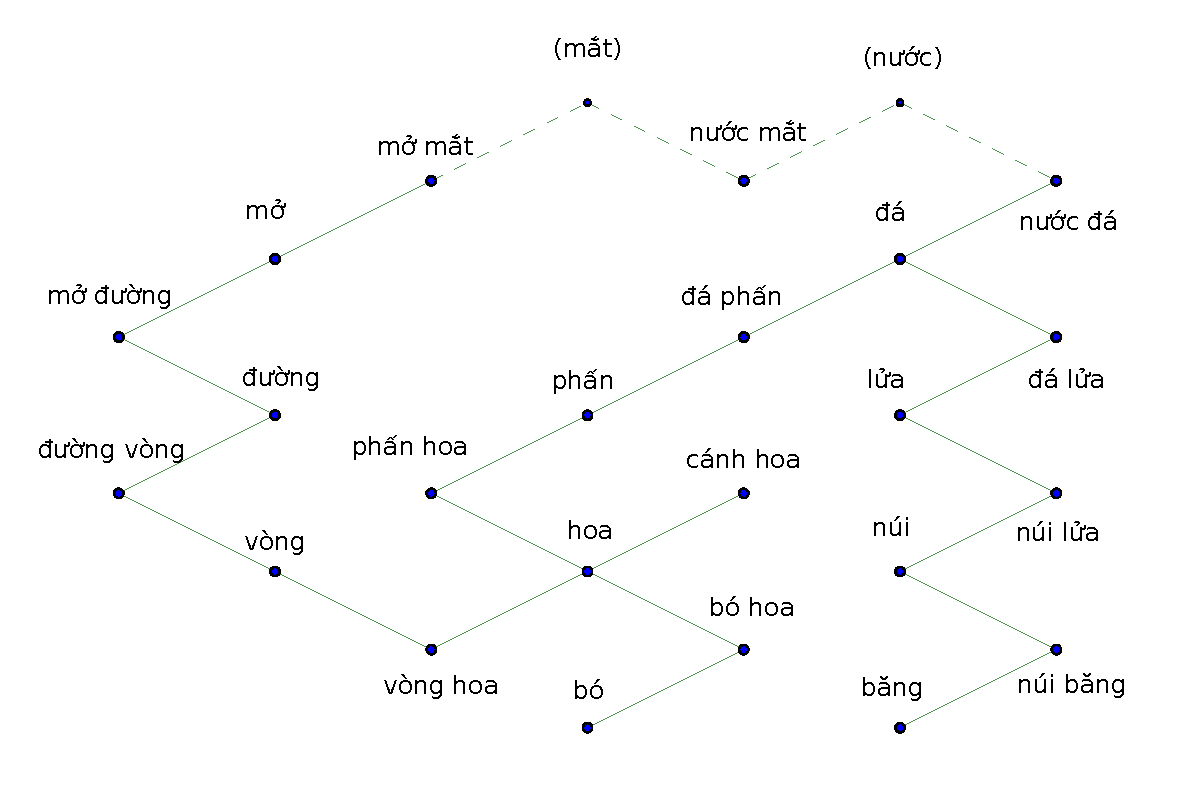
\includegraphics[width= 1\linewidth]{hc-2022-2-2-2-1.pdf}
	\caption{\small\textit{\color{toancuabi}Graph of Vietnamese phrases}}
	\vspace*{-10pt}
\end{figure}
The graph of Vietnamese phrases, we presume, represents connections in \textit{shared meaning} between phrases.
Thus, we connect the English phrases in the same way,
each phrase with another so that one has a meaning that shall be contained by the meaning of the other.
The result is the diagram below.
\begin{figure}[H]
	\vspace*{-5pt}
	\centering
	\captionsetup{labelformat= empty, justification=centering}
	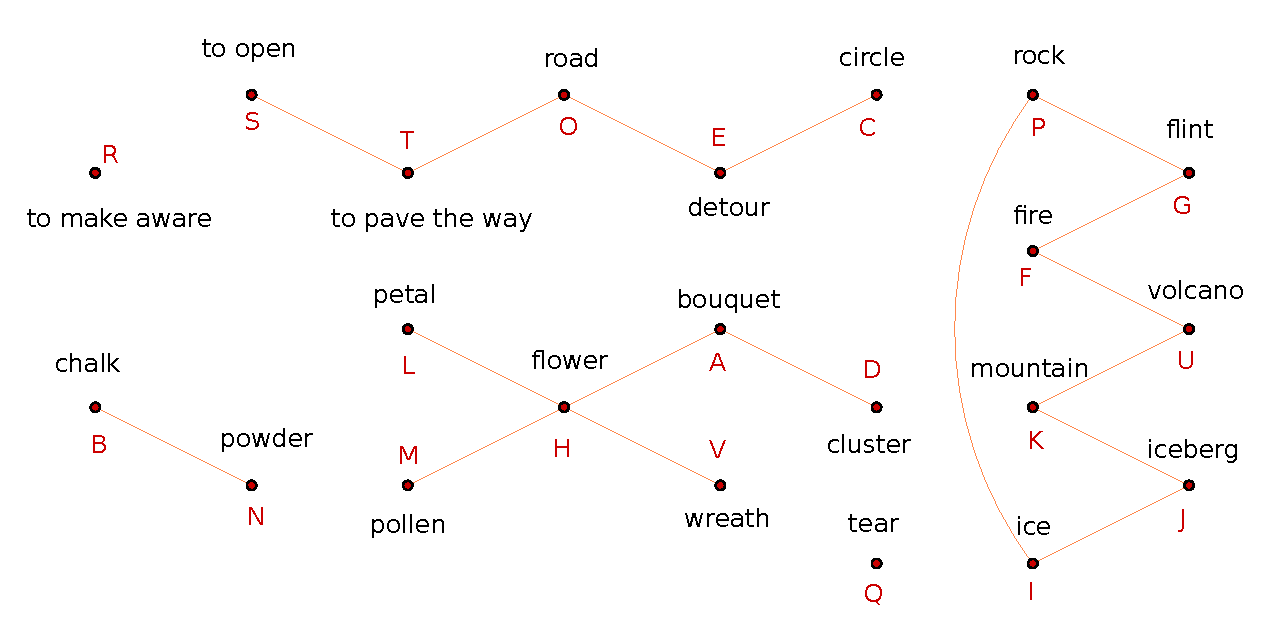
\includegraphics[width= 1\linewidth]{hc-2022-2-2-2-2.pdf}
	\caption{\small\textit{\color{toancuabi}Graph of English phrases}}
	\vspace*{-10pt}
\end{figure}
Comparing the graph, only the $5-vertex$ subgraphs \textit{(phấn hoa, vòng hoa, cánh hoa, bó hoa, hoa)} and
\textit{(bouquet, petal, pollen, wreath, flower),} are \textit{topologically} equivalent, thus \textit{hoa=flower}.
Note that the relation between \textit{pollen} and \textit{powder},
implies that \textit{powder} is \textit{phấn}. The rest of the vertices then can be paired up
\textit{petal -- cánh hoa, bouquet -- bó hoa, pollen -- phấn hoa, wreath -- vòng hoa.}
Therefor \textit{bó -- cluster}, and \textit{chalk -- đá phấn.}
Similarly the paths \textit{(băng -- núi băng -- núi -- núi lửa -- lửa -- đá lửa -- đá -- nước đá)} 
\textit{(ice -- iceberg -- mountain -- volcano -- fire -- flint -- rock)} are very much alike,
in addtion, the relation of \textit{đá -- đá phấn} is similar to \textit{rock -- chalk,}
which make both \textit{nước đá} and \textit{băng} to have the meaning of \textit{ice}.
Similarly the paths \textit{(vòng -- đường vòng -- đường -- mở đường -- mở)} 
\textit{(to open -- to pave the way -- road -- detour -- circle)} are very much alike.
\vskip 0.1cm
Following the reasoning, we can fill the table as shown below.
\end{multicols}
\begin{center}
	\renewcommand{\arraystretch}{1.2}
	\setlength{\tabcolsep}{8pt}
	\begin{tabular}{|c|l|l|c|l|}
		\hline
		$\#$ & Vietnamese & Literal meaning & Answer & English       \\ \hline
		$1 $ & băng       & ice             & I      & ice           \\ \hline
		$2 $ & bó         & cluster         & D      & cluster       \\ \hline
		$3 $ & bó hoa     & flower cluster  & A      & bouquet       \\ \hline
		$4 $ & cánh hoa   & flower wing     & L      & petal         \\ \hline
		$5 $ & đá         & rock            & P      & rock          \\ \hline
		$6 $ & đá lửa     & fire rock       & G      & flint         \\ \hline
		$7 $ & đá phấn    & powder rock     & B      & chalk         \\ \hline
		$8 $ & đường      & road            & O      & road          \\ \hline
		$9 $ & đường vòng & circle road     & E      & detour        \\ \hline
		$10$ & hoa        & flower          & H      & flower        \\ \hline
		$11$ & lửa        & fire            & F      & fire          \\ \hline
		$12$ & mở         & to open         & S      & to open       \\ \hline
		$13$ & mở đường   & to open a road  & T      & to pave a way \\ \hline
		$14$ & mở mắt     & to open eyes    & R      & to make aware \\ \hline
		$15$ & núi        & mountain        & K      & mountain      \\ \hline
		$16$ & núi băng   & ice mountain    & J      & iceberg       \\ \hline
		$17$ & núi lửa    & fire mountain   & U      & volcano       \\ \hline
		$18$ & nước đá    & rock water      & I      & ice           \\ \hline
		$19$ & nước mắt   & eye water       & Q      & tear          \\ \hline
		$20$ & phấn       & powder          & N      & powder        \\ \hline
		$21$ & phấn hoa   & flower powder   & M      & pollen        \\ \hline
		$22$ & vòng       & circle          & C      & circle        \\ \hline
		$23$ & vòng hoa   & flower circle   & V      & wreath        \\ \hline
	\end{tabular}
\end{center}